\documentclass[]{article}
\usepackage{lmodern}
\usepackage{amssymb,amsmath}
\usepackage{ifxetex,ifluatex}
\usepackage{fixltx2e} % provides \textsubscript
\ifnum 0\ifxetex 1\fi\ifluatex 1\fi=0 % if pdftex
  \usepackage[T1]{fontenc}
  \usepackage[utf8]{inputenc}
\else % if luatex or xelatex
  \ifxetex
    \usepackage{mathspec}
  \else
    \usepackage{fontspec}
  \fi
  \defaultfontfeatures{Ligatures=TeX,Scale=MatchLowercase}
\fi
% use upquote if available, for straight quotes in verbatim environments
\IfFileExists{upquote.sty}{\usepackage{upquote}}{}
% use microtype if available
\IfFileExists{microtype.sty}{%
\usepackage{microtype}
\UseMicrotypeSet[protrusion]{basicmath} % disable protrusion for tt fonts
}{}
\usepackage[margin=1in]{geometry}
\usepackage{hyperref}
\hypersetup{unicode=true,
            pdftitle={Hydraulic conductivities of the maize var. B73},
            pdfauthor={Adrien Heymans},
            pdfborder={0 0 0},
            breaklinks=true}
\urlstyle{same}  % don't use monospace font for urls
\usepackage{color}
\usepackage{fancyvrb}
\newcommand{\VerbBar}{|}
\newcommand{\VERB}{\Verb[commandchars=\\\{\}]}
\DefineVerbatimEnvironment{Highlighting}{Verbatim}{commandchars=\\\{\}}
% Add ',fontsize=\small' for more characters per line
\usepackage{framed}
\definecolor{shadecolor}{RGB}{248,248,248}
\newenvironment{Shaded}{\begin{snugshade}}{\end{snugshade}}
\newcommand{\KeywordTok}[1]{\textcolor[rgb]{0.13,0.29,0.53}{\textbf{#1}}}
\newcommand{\DataTypeTok}[1]{\textcolor[rgb]{0.13,0.29,0.53}{#1}}
\newcommand{\DecValTok}[1]{\textcolor[rgb]{0.00,0.00,0.81}{#1}}
\newcommand{\BaseNTok}[1]{\textcolor[rgb]{0.00,0.00,0.81}{#1}}
\newcommand{\FloatTok}[1]{\textcolor[rgb]{0.00,0.00,0.81}{#1}}
\newcommand{\ConstantTok}[1]{\textcolor[rgb]{0.00,0.00,0.00}{#1}}
\newcommand{\CharTok}[1]{\textcolor[rgb]{0.31,0.60,0.02}{#1}}
\newcommand{\SpecialCharTok}[1]{\textcolor[rgb]{0.00,0.00,0.00}{#1}}
\newcommand{\StringTok}[1]{\textcolor[rgb]{0.31,0.60,0.02}{#1}}
\newcommand{\VerbatimStringTok}[1]{\textcolor[rgb]{0.31,0.60,0.02}{#1}}
\newcommand{\SpecialStringTok}[1]{\textcolor[rgb]{0.31,0.60,0.02}{#1}}
\newcommand{\ImportTok}[1]{#1}
\newcommand{\CommentTok}[1]{\textcolor[rgb]{0.56,0.35,0.01}{\textit{#1}}}
\newcommand{\DocumentationTok}[1]{\textcolor[rgb]{0.56,0.35,0.01}{\textbf{\textit{#1}}}}
\newcommand{\AnnotationTok}[1]{\textcolor[rgb]{0.56,0.35,0.01}{\textbf{\textit{#1}}}}
\newcommand{\CommentVarTok}[1]{\textcolor[rgb]{0.56,0.35,0.01}{\textbf{\textit{#1}}}}
\newcommand{\OtherTok}[1]{\textcolor[rgb]{0.56,0.35,0.01}{#1}}
\newcommand{\FunctionTok}[1]{\textcolor[rgb]{0.00,0.00,0.00}{#1}}
\newcommand{\VariableTok}[1]{\textcolor[rgb]{0.00,0.00,0.00}{#1}}
\newcommand{\ControlFlowTok}[1]{\textcolor[rgb]{0.13,0.29,0.53}{\textbf{#1}}}
\newcommand{\OperatorTok}[1]{\textcolor[rgb]{0.81,0.36,0.00}{\textbf{#1}}}
\newcommand{\BuiltInTok}[1]{#1}
\newcommand{\ExtensionTok}[1]{#1}
\newcommand{\PreprocessorTok}[1]{\textcolor[rgb]{0.56,0.35,0.01}{\textit{#1}}}
\newcommand{\AttributeTok}[1]{\textcolor[rgb]{0.77,0.63,0.00}{#1}}
\newcommand{\RegionMarkerTok}[1]{#1}
\newcommand{\InformationTok}[1]{\textcolor[rgb]{0.56,0.35,0.01}{\textbf{\textit{#1}}}}
\newcommand{\WarningTok}[1]{\textcolor[rgb]{0.56,0.35,0.01}{\textbf{\textit{#1}}}}
\newcommand{\AlertTok}[1]{\textcolor[rgb]{0.94,0.16,0.16}{#1}}
\newcommand{\ErrorTok}[1]{\textcolor[rgb]{0.64,0.00,0.00}{\textbf{#1}}}
\newcommand{\NormalTok}[1]{#1}
\usepackage{graphicx,grffile}
\makeatletter
\def\maxwidth{\ifdim\Gin@nat@width>\linewidth\linewidth\else\Gin@nat@width\fi}
\def\maxheight{\ifdim\Gin@nat@height>\textheight\textheight\else\Gin@nat@height\fi}
\makeatother
% Scale images if necessary, so that they will not overflow the page
% margins by default, and it is still possible to overwrite the defaults
% using explicit options in \includegraphics[width, height, ...]{}
\setkeys{Gin}{width=\maxwidth,height=\maxheight,keepaspectratio}
\IfFileExists{parskip.sty}{%
\usepackage{parskip}
}{% else
\setlength{\parindent}{0pt}
\setlength{\parskip}{6pt plus 2pt minus 1pt}
}
\setlength{\emergencystretch}{3em}  % prevent overfull lines
\providecommand{\tightlist}{%
  \setlength{\itemsep}{0pt}\setlength{\parskip}{0pt}}
\setcounter{secnumdepth}{0}
% Redefines (sub)paragraphs to behave more like sections
\ifx\paragraph\undefined\else
\let\oldparagraph\paragraph
\renewcommand{\paragraph}[1]{\oldparagraph{#1}\mbox{}}
\fi
\ifx\subparagraph\undefined\else
\let\oldsubparagraph\subparagraph
\renewcommand{\subparagraph}[1]{\oldsubparagraph{#1}\mbox{}}
\fi

%%% Use protect on footnotes to avoid problems with footnotes in titles
\let\rmarkdownfootnote\footnote%
\def\footnote{\protect\rmarkdownfootnote}

%%% Change title format to be more compact
\usepackage{titling}

% Create subtitle command for use in maketitle
\newcommand{\subtitle}[1]{
  \posttitle{
    \begin{center}\large#1\end{center}
    }
}

\setlength{\droptitle}{-2em}

  \title{Hydraulic conductivities of the maize var. B73}
    \pretitle{\vspace{\droptitle}\centering\huge}
  \posttitle{\par}
    \author{Adrien Heymans}
    \preauthor{\centering\large\emph}
  \postauthor{\par}
      \predate{\centering\large\emph}
  \postdate{\par}
    \date{30/11/2020}


\begin{document}
\maketitle

\subsection{Protocol to get the hydraulic conductivities along the root
axes of maize
root.}\label{protocol-to-get-the-hydraulic-conductivities-along-the-root-axes-of-maize-root.}

The results of coupling GRANAR with MECHA is the estimation of the
hydraulic conductivities of a root. GRANAR will generate root cross
section anatomy. MECHA will use the synthetic root cross section to
calculate the radial conductivities (Kr) and the axial conductance (Kx).

To access the information needed to run GRANAR, it requires free-hand
section or permanent root cross section. Staining the cross section will
allow to spot the different apoplastic barriers.

In this example, free-hand section were stain with aqueouse solution of
berberin (1h) and post-stain with analine blue (30min).

\begin{figure}
\centering
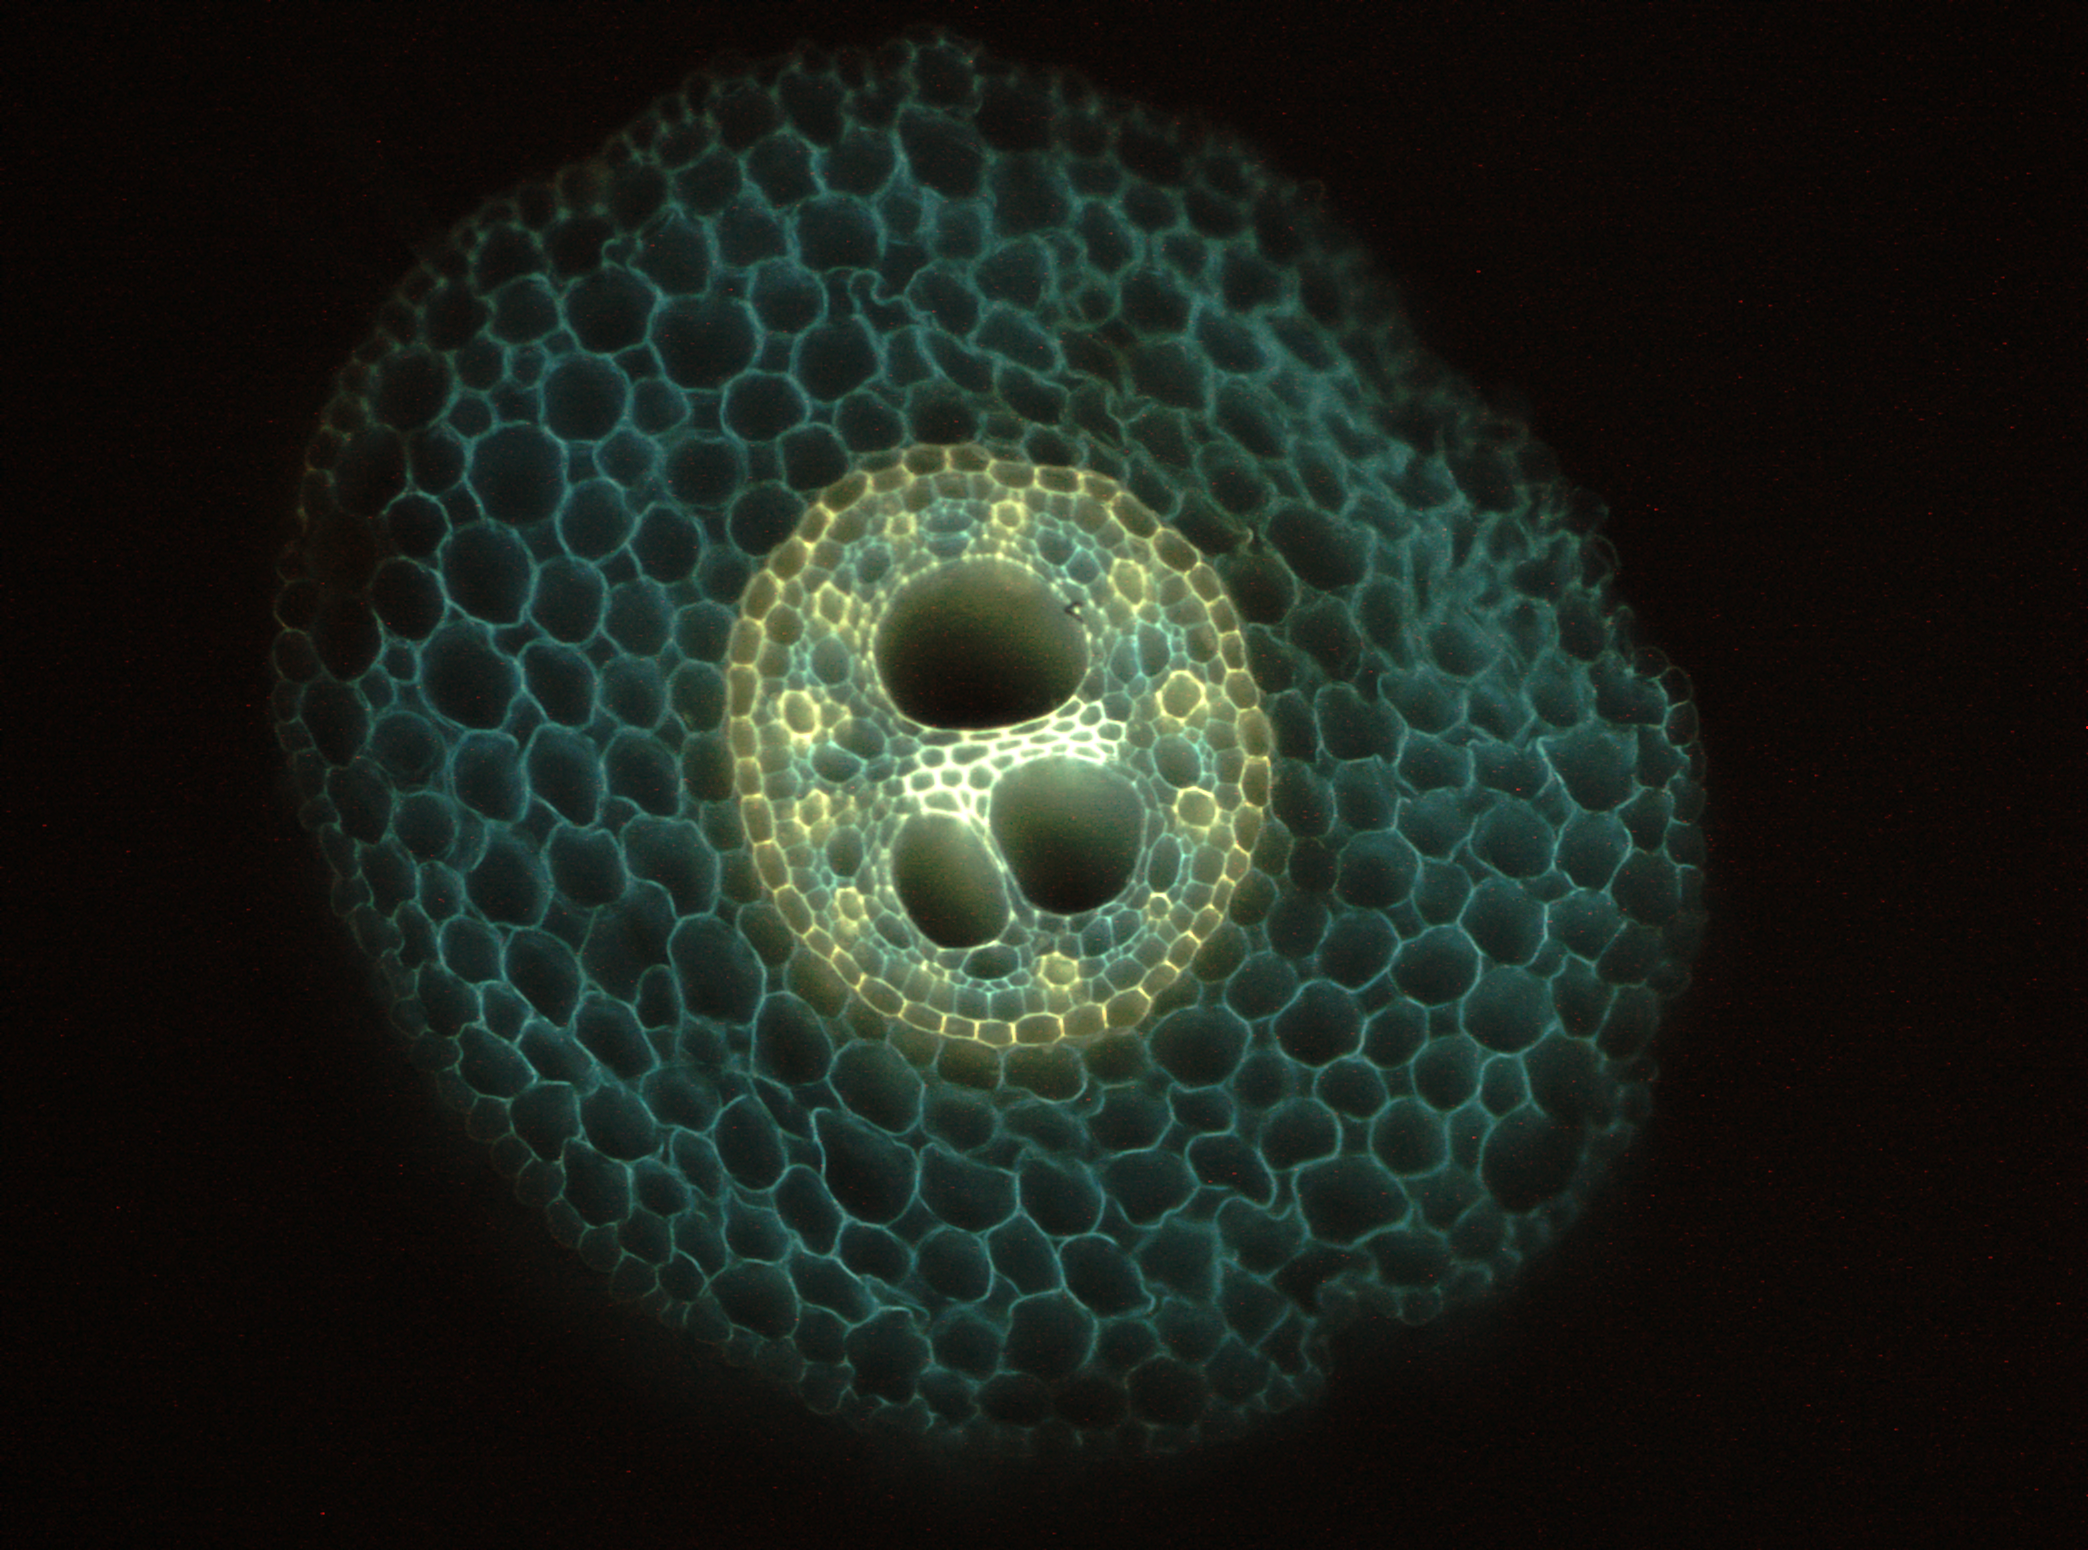
\includegraphics{Image_000334.png}
\caption{Basal root at 15cm from the tip stain with berberin and
post-stain with analine blue}
\end{figure}

\begin{verbatim}
## Warning: package 'tidyverse' was built under R version 3.5.3
\end{verbatim}

\begin{verbatim}
## Warning: package 'ggplot2' was built under R version 3.5.3
\end{verbatim}

\begin{verbatim}
## Warning: package 'tibble' was built under R version 3.5.3
\end{verbatim}

\begin{verbatim}
## Warning: package 'tidyr' was built under R version 3.5.3
\end{verbatim}

\begin{verbatim}
## Warning: package 'readr' was built under R version 3.5.3
\end{verbatim}

\begin{verbatim}
## Warning: package 'purrr' was built under R version 3.5.3
\end{verbatim}

\begin{verbatim}
## Warning: package 'dplyr' was built under R version 3.5.3
\end{verbatim}

\begin{verbatim}
## Warning: package 'stringr' was built under R version 3.5.3
\end{verbatim}

\begin{verbatim}
## Warning: package 'forcats' was built under R version 3.5.3
\end{verbatim}

\begin{verbatim}
## Warning: package 'readxl' was built under R version 3.5.3
\end{verbatim}

\begin{verbatim}
## Warning: package 'plyr' was built under R version 3.5.3
\end{verbatim}

\begin{verbatim}
## Warning: package 'deldir' was built under R version 3.5.3
\end{verbatim}

\begin{verbatim}
## Warning: package 'alphahull' was built under R version 3.5.3
\end{verbatim}

\begin{verbatim}
## Warning: package 'xml2' was built under R version 3.5.3
\end{verbatim}

\subsubsection{Loading experimental
data}\label{loading-experimental-data}

\begin{Shaded}
\begin{Highlighting}[]
\NormalTok{root_name <-}\StringTok{ }\KeywordTok{c}\NormalTok{(}\StringTok{"SBR"}\NormalTok{, }\StringTok{"Tap"}\NormalTok{, }\StringTok{"Basal"}\NormalTok{, }\StringTok{"LAT"}\NormalTok{, }\StringTok{"LAT_A"}\NormalTok{)}

\NormalTok{Data_params <-}\StringTok{ }\KeywordTok{read_excel}\NormalTok{(}\StringTok{"Data_params.xlsx"}\NormalTok{)}\OperatorTok
\StringTok{  }\KeywordTok{as.tibble}\NormalTok{()}
\NormalTok{Data_params}\OperatorTok{$}\NormalTok{cell[Data_params}\OperatorTok{$}\NormalTok{Root_id }\OperatorTok{==}\StringTok{ "05_01"} \OperatorTok{&}\StringTok{ }\NormalTok{Data_params}\OperatorTok{$}\NormalTok{tissue }\OperatorTok{==}\StringTok{ "xylem"} \OperatorTok{&}\StringTok{ }\OperatorTok{!}\KeywordTok{is.na}\NormalTok{(Data_params}\OperatorTok{$}\NormalTok{cell)] <-}\StringTok{ }\NormalTok{Data_params}\OperatorTok{$}\NormalTok{cell[Data_params}\OperatorTok{$}\NormalTok{Root_id }\OperatorTok{==}\StringTok{ "05_01"} \OperatorTok{&}\StringTok{ }\NormalTok{Data_params}\OperatorTok{$}\NormalTok{tissue }\OperatorTok{==}\StringTok{ "xylem"} \OperatorTok{&}\StringTok{ }\OperatorTok{!}\KeywordTok{is.na}\NormalTok{(Data_params}\OperatorTok{$}\NormalTok{cell)]}\OperatorTok{*}\DecValTok{2}
\NormalTok{params <-}\StringTok{ }\KeywordTok{read_param_xml}\NormalTok{(}\StringTok{"www/Zea_mays_B73_S_01.xml"}\NormalTok{)}

\CommentTok{# number of time the generation of anatomies will be replicated.}
\NormalTok{n_rep <-}\StringTok{ }\DecValTok{2} \CommentTok{# always >1}
\end{Highlighting}
\end{Shaded}

\begin{Shaded}
\begin{Highlighting}[]
\NormalTok{Data_params}\OperatorTok
\StringTok{  }\KeywordTok{filter}\NormalTok{(tissue }\OperatorTok\StringTok{ }\KeywordTok{c}\NormalTok{(}\StringTok{"proto"}\NormalTok{, }\StringTok{"xylem"}\NormalTok{),}
         \OperatorTok{!}\KeywordTok{is.na}\NormalTok{(tissue),}
\NormalTok{         tissue }\OperatorTok{!=}\StringTok{ "aer"}\NormalTok{)}\OperatorTok
\StringTok{  }\KeywordTok{ggplot}\NormalTok{(}\KeywordTok{aes}\NormalTok{(dist, cell))}\OperatorTok{+}
\StringTok{  }\KeywordTok{geom_point}\NormalTok{(}\DataTypeTok{alpha =} \FloatTok{0.2}\NormalTok{, }\KeywordTok{aes}\NormalTok{(}\DataTypeTok{colour =}\NormalTok{ Root))}\OperatorTok{+}
\StringTok{  }\KeywordTok{geom_smooth}\NormalTok{(}\DataTypeTok{method =} \StringTok{"lm"}\NormalTok{, }\KeywordTok{aes}\NormalTok{(}\DataTypeTok{colour =}\NormalTok{ Root))}\OperatorTok{+}
\StringTok{  }\KeywordTok{facet_wrap}\NormalTok{(}\OperatorTok{~}\NormalTok{tissue)}\OperatorTok{+}
\StringTok{  }\KeywordTok{ylab}\NormalTok{(}\StringTok{"Cell size [戼㸵m]"}\NormalTok{)}\OperatorTok{+}
\StringTok{  }\KeywordTok{xlab}\NormalTok{(}\StringTok{"distance from the tip [cm]"}\NormalTok{)}\OperatorTok{+}
\StringTok{  }\NormalTok{viridis}\OperatorTok{::}\KeywordTok{scale_colour_viridis}\NormalTok{(}\DataTypeTok{discrete =}\NormalTok{ T)}
\end{Highlighting}
\end{Shaded}

\begin{verbatim}
## `geom_smooth()` using formula 'y ~ x'
\end{verbatim}

\begin{verbatim}
## Warning: Removed 21 rows containing non-finite values (stat_smooth).
\end{verbatim}

\begin{verbatim}
## Warning: Removed 21 rows containing missing values (geom_point).
\end{verbatim}

\includegraphics{Protocol_hydro_map_files/figure-latex/unnamed-chunk-2-1.pdf}

\begin{Shaded}
\begin{Highlighting}[]
\NormalTok{Data_params}\OperatorTok
\StringTok{  }\KeywordTok{filter}\NormalTok{(tissue }\OperatorTok\StringTok{ }\KeywordTok{c}\NormalTok{(}\StringTok{"cortex"}\NormalTok{))}\OperatorTok
\StringTok{  }\KeywordTok{ggplot}\NormalTok{(}\KeywordTok{aes}\NormalTok{(Root, layer))}\OperatorTok{+}
\StringTok{  }\KeywordTok{geom_boxplot}\NormalTok{(}\KeywordTok{aes}\NormalTok{(}\DataTypeTok{colour =}\NormalTok{ Root))}\OperatorTok{+}
\StringTok{  }\KeywordTok{facet_grid}\NormalTok{(}\OperatorTok{~}\NormalTok{tissue)}\OperatorTok{+}
\StringTok{  }\KeywordTok{ylab}\NormalTok{(}\StringTok{"layer width [戼㸵m]"}\NormalTok{)}\OperatorTok{+}
\StringTok{  }\KeywordTok{xlab}\NormalTok{(}\StringTok{"distance from the tip [cm]"}\NormalTok{)}\OperatorTok{+}
\StringTok{  }\NormalTok{viridis}\OperatorTok{::}\KeywordTok{scale_colour_viridis}\NormalTok{(}\DataTypeTok{discrete =}\NormalTok{ T)}
\end{Highlighting}
\end{Shaded}

\begin{verbatim}
## Warning: Removed 2 rows containing non-finite values (stat_boxplot).
\end{verbatim}

\includegraphics{Protocol_hydro_map_files/figure-latex/unnamed-chunk-2-2.pdf}

\begin{Shaded}
\begin{Highlighting}[]
\NormalTok{Data_params}\OperatorTok
\StringTok{  }\KeywordTok{filter}\NormalTok{(tissue }\OperatorTok{==}\StringTok{ "xylem"}\NormalTok{,}
         \OperatorTok{!}\KeywordTok{is.na}\NormalTok{(tissue))}\OperatorTok
\StringTok{  }\KeywordTok{ggplot}\NormalTok{(}\KeywordTok{aes}\NormalTok{(dist, cell))}\OperatorTok{+}
\StringTok{  }\KeywordTok{geom_point}\NormalTok{(}\DataTypeTok{alpha =} \FloatTok{0.2}\NormalTok{, }\KeywordTok{aes}\NormalTok{(}\DataTypeTok{colour =}\NormalTok{ Root))}\OperatorTok{+}
\StringTok{  }\KeywordTok{geom_smooth}\NormalTok{(}\DataTypeTok{method =} \StringTok{"lm"}\NormalTok{, }\KeywordTok{aes}\NormalTok{(}\DataTypeTok{colour =}\NormalTok{ Root))}\OperatorTok{+}
\StringTok{  }\KeywordTok{facet_wrap}\NormalTok{(}\OperatorTok{~}\NormalTok{tissue)}\OperatorTok{+}
\StringTok{  }\KeywordTok{ylab}\NormalTok{(}\StringTok{"Cell size [戼㸵m]"}\NormalTok{)}\OperatorTok{+}
\StringTok{  }\KeywordTok{xlab}\NormalTok{(}\StringTok{"distance from the tip [cm]"}\NormalTok{)}\OperatorTok{+}
\StringTok{  }\NormalTok{viridis}\OperatorTok{::}\KeywordTok{scale_colour_viridis}\NormalTok{(}\DataTypeTok{discrete =}\NormalTok{ T)}
\end{Highlighting}
\end{Shaded}

\begin{verbatim}
## `geom_smooth()` using formula 'y ~ x'
\end{verbatim}

\begin{verbatim}
## Warning: Removed 3 rows containing non-finite values (stat_smooth).
\end{verbatim}

\begin{verbatim}
## Warning: Removed 3 rows containing missing values (geom_point).
\end{verbatim}

\includegraphics{Protocol_hydro_map_files/figure-latex/unnamed-chunk-2-3.pdf}

\begin{Shaded}
\begin{Highlighting}[]
\NormalTok{cor_ma_tmp <-}\StringTok{ }\NormalTok{Data_params}\OperatorTok
\StringTok{  }\KeywordTok{filter}\NormalTok{(tissue }\OperatorTok\StringTok{ }\KeywordTok{c}\NormalTok{(}\StringTok{"xylem"}\NormalTok{))}\OperatorTok
\StringTok{  }\NormalTok{dplyr}\OperatorTok{::}\KeywordTok{group_by}\NormalTok{(Image)}\OperatorTok
\StringTok{  }\NormalTok{dplyr}\OperatorTok{::}\KeywordTok{summarise}\NormalTok{(}\DataTypeTok{xylem_size =} \KeywordTok{mean}\NormalTok{(cell))}\OperatorTok
\StringTok{  }\KeywordTok{ungroup}\NormalTok{()}
\NormalTok{cor_ms_tmp <-}\StringTok{ }\NormalTok{Data_params}\OperatorTok
\StringTok{  }\KeywordTok{filter}\NormalTok{(tissue }\OperatorTok\StringTok{ }\KeywordTok{c}\NormalTok{(}\StringTok{"stele"}\NormalTok{))}\OperatorTok
\StringTok{  }\NormalTok{dplyr}\OperatorTok{::}\KeywordTok{group_by}\NormalTok{(Image)}\OperatorTok
\StringTok{  }\NormalTok{dplyr}\OperatorTok{::}\KeywordTok{summarise}\NormalTok{(}\DataTypeTok{stele_size =} \KeywordTok{mean}\NormalTok{(layer))}\OperatorTok
\StringTok{  }\KeywordTok{ungroup}\NormalTok{()}

\NormalTok{cor <-}\StringTok{ }\KeywordTok{merge}\NormalTok{(cor_ma_tmp, cor_ms_tmp, }\DataTypeTok{by =} \StringTok{"Image"}\NormalTok{)}
\NormalTok{cor }\OperatorTok
\StringTok{  }\KeywordTok{ggplot}\NormalTok{()}\OperatorTok{+}
\StringTok{  }\KeywordTok{geom_point}\NormalTok{(}\KeywordTok{aes}\NormalTok{(stele_size, xylem_size))}
\end{Highlighting}
\end{Shaded}

\begin{verbatim}
## Warning: Removed 2 rows containing missing values (geom_point).
\end{verbatim}

\includegraphics{Protocol_hydro_map_files/figure-latex/unnamed-chunk-3-1.pdf}

\begin{Shaded}
\begin{Highlighting}[]
\KeywordTok{ggpairs}\NormalTok{(cor}\OperatorTok\KeywordTok{select}\NormalTok{(}\OperatorTok{-}\NormalTok{Image))}
\end{Highlighting}
\end{Shaded}

\begin{verbatim}
## Warning: Removed 1 rows containing non-finite values (stat_density).
\end{verbatim}

\begin{verbatim}
## Warning in (function (data, mapping, alignPercent = 0.6, method = "pearson", :
## Removed 2 rows containing missing values
\end{verbatim}

\begin{verbatim}
## Warning: Removed 2 rows containing missing values (geom_point).
\end{verbatim}

\begin{verbatim}
## Warning: Removed 1 rows containing non-finite values (stat_density).
\end{verbatim}

\includegraphics{Protocol_hydro_map_files/figure-latex/unnamed-chunk-3-2.pdf}

\begin{Shaded}
\begin{Highlighting}[]
\NormalTok{stelar <-}\StringTok{ }\NormalTok{Data_params}\OperatorTok
\StringTok{  }\KeywordTok{filter}\NormalTok{(tissue }\OperatorTok\StringTok{ }\KeywordTok{c}\NormalTok{(}\StringTok{"stele"}\NormalTok{))}

\NormalTok{stelar}\OperatorTok
\StringTok{  }\KeywordTok{ggplot}\NormalTok{(}\KeywordTok{aes}\NormalTok{(dist, layer))}\OperatorTok{+}
\StringTok{  }\KeywordTok{geom_point}\NormalTok{(}\KeywordTok{aes}\NormalTok{(}\DataTypeTok{colour =}\NormalTok{ Root))}\OperatorTok{+}
\StringTok{  }\KeywordTok{geom_smooth}\NormalTok{(}\KeywordTok{aes}\NormalTok{(}\DataTypeTok{colour =}\NormalTok{ Root), }\DataTypeTok{method =} \StringTok{"lm"}\NormalTok{)}\OperatorTok{+}
\StringTok{  }\KeywordTok{facet_grid}\NormalTok{(}\OperatorTok{~}\NormalTok{tissue)}\OperatorTok{+}
\StringTok{  }\NormalTok{viridis}\OperatorTok{::}\KeywordTok{scale_colour_viridis}\NormalTok{(}\DataTypeTok{discrete=}\NormalTok{ T)}
\end{Highlighting}
\end{Shaded}

\begin{verbatim}
## `geom_smooth()` using formula 'y ~ x'
\end{verbatim}

\begin{verbatim}
## Warning: Removed 2 rows containing non-finite values (stat_smooth).
\end{verbatim}

\begin{verbatim}
## Warning: Removed 2 rows containing missing values (geom_point).
\end{verbatim}

\includegraphics{Protocol_hydro_map_files/figure-latex/unnamed-chunk-4-1.pdf}

\begin{Shaded}
\begin{Highlighting}[]
\NormalTok{xylem <-}\StringTok{ }\NormalTok{Data_params}\OperatorTok
\StringTok{  }\KeywordTok{filter}\NormalTok{(tissue }\OperatorTok\StringTok{ }\KeywordTok{c}\NormalTok{(}\StringTok{"xylem"}\NormalTok{))}

\NormalTok{xylem }\OperatorTok
\StringTok{  }\KeywordTok{ggplot}\NormalTok{(}\KeywordTok{aes}\NormalTok{(dist, cell, }\DataTypeTok{colour =}\NormalTok{ Root))}\OperatorTok{+}
\StringTok{  }\KeywordTok{geom_point}\NormalTok{()}\OperatorTok{+}
\StringTok{  }\KeywordTok{geom_smooth}\NormalTok{(}\DataTypeTok{method =} \StringTok{"lm"}\NormalTok{)}\OperatorTok{+}
\StringTok{  }\NormalTok{viridis}\OperatorTok{::}\KeywordTok{scale_colour_viridis}\NormalTok{(}\DataTypeTok{discrete=}\NormalTok{ T)}
\end{Highlighting}
\end{Shaded}

\begin{verbatim}
## `geom_smooth()` using formula 'y ~ x'
\end{verbatim}

\begin{verbatim}
## Warning: Removed 3 rows containing non-finite values (stat_smooth).
\end{verbatim}

\begin{verbatim}
## Warning: Removed 3 rows containing missing values (geom_point).
\end{verbatim}

\includegraphics{Protocol_hydro_map_files/figure-latex/unnamed-chunk-4-2.pdf}

\begin{Shaded}
\begin{Highlighting}[]
\NormalTok{xylem }\OperatorTok
\StringTok{  }\KeywordTok{ggplot}\NormalTok{(}\KeywordTok{aes}\NormalTok{(dist, layer, }\DataTypeTok{colour =}\NormalTok{ Root))}\OperatorTok{+}
\StringTok{  }\KeywordTok{geom_point}\NormalTok{()}\OperatorTok{+}
\StringTok{  }\KeywordTok{geom_smooth}\NormalTok{(}\DataTypeTok{method =} \StringTok{"lm"}\NormalTok{)}\OperatorTok{+}
\StringTok{  }\NormalTok{viridis}\OperatorTok{::}\KeywordTok{scale_colour_viridis}\NormalTok{(}\DataTypeTok{discrete=}\NormalTok{ T)}
\end{Highlighting}
\end{Shaded}

\begin{verbatim}
## `geom_smooth()` using formula 'y ~ x'
\end{verbatim}

\begin{verbatim}
## Warning: Removed 298 rows containing non-finite values (stat_smooth).
\end{verbatim}

\begin{verbatim}
## Warning: Removed 298 rows containing missing values (geom_point).
\end{verbatim}

\includegraphics{Protocol_hydro_map_files/figure-latex/unnamed-chunk-4-3.pdf}

\begin{Shaded}
\begin{Highlighting}[]
\NormalTok{cortex <-}\StringTok{ }\NormalTok{Data_params}\OperatorTok
\StringTok{  }\KeywordTok{filter}\NormalTok{(tissue }\OperatorTok\StringTok{ }\KeywordTok{c}\NormalTok{(}\StringTok{"cortex"}\NormalTok{))}

\NormalTok{cortex }\OperatorTok
\StringTok{  }\KeywordTok{ggplot}\NormalTok{(}\KeywordTok{aes}\NormalTok{(dist, layer, }\DataTypeTok{colour =}\NormalTok{ Root))}\OperatorTok{+}
\StringTok{  }\KeywordTok{geom_point}\NormalTok{()}\OperatorTok{+}
\StringTok{  }\KeywordTok{geom_smooth}\NormalTok{(}\DataTypeTok{method =} \StringTok{"lm"}\NormalTok{)}\OperatorTok{+}
\StringTok{  }\KeywordTok{ylab}\NormalTok{(}\StringTok{"cortex width"}\NormalTok{)}\OperatorTok{+}
\StringTok{  }\NormalTok{viridis}\OperatorTok{::}\KeywordTok{scale_colour_viridis}\NormalTok{(}\DataTypeTok{discrete=}\NormalTok{ T)}
\end{Highlighting}
\end{Shaded}

\begin{verbatim}
## `geom_smooth()` using formula 'y ~ x'
\end{verbatim}

\begin{verbatim}
## Warning: Removed 6 rows containing non-finite values (stat_smooth).
\end{verbatim}

\begin{verbatim}
## Warning: Removed 6 rows containing missing values (geom_point).
\end{verbatim}

\includegraphics{Protocol_hydro_map_files/figure-latex/unnamed-chunk-4-4.pdf}

\begin{Shaded}
\begin{Highlighting}[]
\NormalTok{rom <-}\StringTok{ }\KeywordTok{read_excel}\NormalTok{(}\StringTok{"Root_maturation.xlsx"}\NormalTok{)}\OperatorTok
\StringTok{  }\KeywordTok{as.tibble}\NormalTok{()}

\NormalTok{Data_params}\OperatorTok
\StringTok{  }\KeywordTok{filter}\NormalTok{(}\OperatorTok{!}\KeywordTok{is.na}\NormalTok{(Xyl_m) )}\OperatorTok
\StringTok{  }\KeywordTok{ggplot}\NormalTok{()}\OperatorTok{+}
\StringTok{  }\KeywordTok{geom_point}\NormalTok{(}\KeywordTok{aes}\NormalTok{(dist, Xyl_m, }\DataTypeTok{colour =}\NormalTok{ Root))}\OperatorTok{+}
\StringTok{  }\KeywordTok{geom_line}\NormalTok{(}\KeywordTok{aes}\NormalTok{(dist, Xyl, }\DataTypeTok{colour =}\NormalTok{ Root), }\DataTypeTok{size =} \DecValTok{1}\NormalTok{, }\DataTypeTok{alpha =} \FloatTok{0.8}\NormalTok{, }\DataTypeTok{data =}\NormalTok{ rom)}\OperatorTok{+}
\StringTok{  }\KeywordTok{facet_wrap}\NormalTok{(}\OperatorTok{~}\NormalTok{Root, }\DataTypeTok{scale =} \StringTok{"free"}\NormalTok{)}\OperatorTok{+}
\StringTok{  }\NormalTok{viridis}\OperatorTok{::}\KeywordTok{scale_colour_viridis}\NormalTok{(}\DataTypeTok{discrete=}\NormalTok{ T)}
\end{Highlighting}
\end{Shaded}

\begin{verbatim}
## Warning: Removed 1 rows containing missing values (geom_point).
\end{verbatim}

\includegraphics{Protocol_hydro_map_files/figure-latex/unnamed-chunk-5-1.pdf}

\begin{Shaded}
\begin{Highlighting}[]
\NormalTok{Data_params}\OperatorTok
\StringTok{  }\KeywordTok{filter}\NormalTok{(}\OperatorTok{!}\KeywordTok{is.na}\NormalTok{(Xyl_m), Root_id }\OperatorTok{!=}\StringTok{ "14_01"}\NormalTok{ )}\OperatorTok\StringTok{ }\CommentTok{# outliers}
\StringTok{  }\KeywordTok{ggplot}\NormalTok{()}\OperatorTok{+}
\StringTok{  }\KeywordTok{geom_point}\NormalTok{(}\KeywordTok{aes}\NormalTok{(dist, }\OperatorTok{-}\NormalTok{Apo, }\DataTypeTok{colour =}\NormalTok{ Root))}\OperatorTok{+}
\StringTok{  }\KeywordTok{geom_line}\NormalTok{(}\KeywordTok{aes}\NormalTok{(dist, }\OperatorTok{-}\NormalTok{Apo, }\DataTypeTok{colour =}\NormalTok{ Root), }\DataTypeTok{size =} \DecValTok{1}\NormalTok{, }\DataTypeTok{alpha =} \FloatTok{0.5}\NormalTok{, }\DataTypeTok{data =}\NormalTok{ rom}\OperatorTok\KeywordTok{filter}\NormalTok{(}\OperatorTok{!}\KeywordTok{is.na}\NormalTok{(Apo)))}\OperatorTok{+}
\StringTok{  }\KeywordTok{facet_wrap}\NormalTok{(}\OperatorTok{~}\NormalTok{Root, }\DataTypeTok{scale =} \StringTok{"free"}\NormalTok{)}\OperatorTok{+}
\StringTok{  }\NormalTok{viridis}\OperatorTok{::}\KeywordTok{scale_colour_viridis}\NormalTok{(}\DataTypeTok{discrete=}\NormalTok{ T)}
\end{Highlighting}
\end{Shaded}

\begin{verbatim}
## Warning: Removed 1 rows containing missing values (geom_point).
\end{verbatim}

\includegraphics{Protocol_hydro_map_files/figure-latex/unnamed-chunk-5-2.pdf}

\begin{Shaded}
\begin{Highlighting}[]
\CommentTok{# Prepare data}
\NormalTok{Data <-}\StringTok{ }\NormalTok{Data_params}\OperatorTok
\StringTok{  }\NormalTok{dplyr}\OperatorTok{::}\KeywordTok{group_by}\NormalTok{(Image, tissue, dist, Root, Root_id)}\OperatorTok
\StringTok{  }\NormalTok{dplyr}\OperatorTok{::}\KeywordTok{summarise}\NormalTok{(}\DataTypeTok{cell =} \KeywordTok{mean}\NormalTok{(cell, }\DataTypeTok{na.rm =}\NormalTok{ T),}
                   \DataTypeTok{layer =} \KeywordTok{mean}\NormalTok{(layer, }\DataTypeTok{na.rm =}\NormalTok{ T))}\OperatorTok
\StringTok{  }\KeywordTok{ungroup}\NormalTok{()}\OperatorTok
\StringTok{  }\KeywordTok{filter}\NormalTok{(}\OperatorTok{!}\KeywordTok{is.na}\NormalTok{(tissue))  }

\NormalTok{stele =}\StringTok{ }\NormalTok{CT =}\StringTok{ }\NormalTok{nX =}\StringTok{ }\NormalTok{xylem =}\StringTok{ }\NormalTok{CF <-}\StringTok{ }\OtherTok{NULL}

\ControlFlowTok{for}\NormalTok{ (im }\ControlFlowTok{in} \KeywordTok{unique}\NormalTok{(Data}\OperatorTok{$}\NormalTok{Image)) \{}
  \CommentTok{# Get the total diameter of the root}
  
\NormalTok{  tmp <-}\StringTok{ }\NormalTok{Data}\OperatorTok
\StringTok{    }\KeywordTok{filter}\NormalTok{(Image }\OperatorTok{==}\StringTok{ }\NormalTok{im)}
  \ControlFlowTok{if}\NormalTok{(}\KeywordTok{nrow}\NormalTok{(tmp) }\OperatorTok{==}\StringTok{ }\DecValTok{8}\NormalTok{)\{}
    
\NormalTok{    tot <-}\StringTok{ }\NormalTok{tmp}\OperatorTok{$}\NormalTok{cell[tmp}\OperatorTok{$}\NormalTok{tissue }\OperatorTok{==}\StringTok{ "endo"}\NormalTok{]}\OperatorTok{+}
\StringTok{      }\NormalTok{tmp}\OperatorTok{$}\NormalTok{cell[tmp}\OperatorTok{$}\NormalTok{tissue }\OperatorTok{==}\StringTok{ "pericycle"}\NormalTok{]}\OperatorTok{+}
\StringTok{      }\NormalTok{tmp}\OperatorTok{$}\NormalTok{cell[tmp}\OperatorTok{$}\NormalTok{tissue }\OperatorTok{==}\StringTok{ "exo"}\NormalTok{]}\OperatorTok{+}
\StringTok{      }\NormalTok{tmp}\OperatorTok{$}\NormalTok{cell[tmp}\OperatorTok{$}\NormalTok{tissue }\OperatorTok{==}\StringTok{ "epi"}\NormalTok{]}\OperatorTok{+}
\StringTok{      }\NormalTok{tmp}\OperatorTok{$}\NormalTok{layer[tmp}\OperatorTok{$}\NormalTok{tissue }\OperatorTok{==}\StringTok{ "stele"}\NormalTok{]}\OperatorTok{/}\DecValTok{2}\OperatorTok{+}
\StringTok{      }\NormalTok{tmp}\OperatorTok{$}\NormalTok{layer[tmp}\OperatorTok{$}\NormalTok{tissue }\OperatorTok{==}\StringTok{ "cortex"}\NormalTok{]}
    
\NormalTok{    total <-}\StringTok{ }\KeywordTok{tibble}\NormalTok{(}\DataTypeTok{Image =}\NormalTok{ im, }
                    \DataTypeTok{tissue =} \KeywordTok{c}\NormalTok{(}\StringTok{"total"}\NormalTok{),}
                    \DataTypeTok{cell =} \OtherTok{NA}\NormalTok{, }
                    \DataTypeTok{layer =}\NormalTok{ tot, }
                    \DataTypeTok{dist =} \KeywordTok{unique}\NormalTok{(tmp}\OperatorTok{$}\NormalTok{dist), }
                    \DataTypeTok{Root =} \KeywordTok{unique}\NormalTok{(tmp}\OperatorTok{$}\NormalTok{Root),}
                    \DataTypeTok{Root_id =} \KeywordTok{unique}\NormalTok{(tmp}\OperatorTok{$}\NormalTok{Root_id))}
\NormalTok{    stele <-}\StringTok{ }\KeywordTok{cbind}\NormalTok{(stele, tmp}\OperatorTok{$}\NormalTok{layer[tmp}\OperatorTok{$}\NormalTok{tissue }\OperatorTok{==}\StringTok{ "stele"}\NormalTok{]}\OperatorTok{/}\DecValTok{2}\OperatorTok{+}\NormalTok{tmp}\OperatorTok{$}\NormalTok{cell[tmp}\OperatorTok{$}\NormalTok{tissue }\OperatorTok{==}\StringTok{ "endo"}\NormalTok{]}\OperatorTok{+}
\StringTok{      }\NormalTok{tmp}\OperatorTok{$}\NormalTok{cell[tmp}\OperatorTok{$}\NormalTok{tissue }\OperatorTok{==}\StringTok{ "pericycle"}\NormalTok{])}
\NormalTok{    CF <-}\StringTok{ }\KeywordTok{cbind}\NormalTok{(CF, tmp}\OperatorTok{$}\NormalTok{layer[tmp}\OperatorTok{$}\NormalTok{tissue }\OperatorTok{==}\StringTok{ "cortex"}\NormalTok{]}\OperatorTok{/}\NormalTok{tmp}\OperatorTok{$}\NormalTok{cell[tmp}\OperatorTok{$}\NormalTok{tissue }\OperatorTok{==}\StringTok{ "cortex"}\NormalTok{])}
\NormalTok{    CT <-}\StringTok{ }\KeywordTok{cbind}\NormalTok{(CT, tot)}
\NormalTok{    nX <-}\StringTok{ }\KeywordTok{cbind}\NormalTok{(nX, tmp}\OperatorTok{$}\NormalTok{layer[tmp}\OperatorTok{$}\NormalTok{tissue }\OperatorTok{==}\StringTok{ "xylem"}\NormalTok{] )}
\NormalTok{    xylem <-}\StringTok{ }\KeywordTok{cbind}\NormalTok{(xylem, tmp}\OperatorTok{$}\NormalTok{cell[tmp}\OperatorTok{$}\NormalTok{tissue }\OperatorTok{==}\StringTok{ "xylem"}\NormalTok{])}
    
\NormalTok{    Data <-}\StringTok{ }\KeywordTok{rbind}\NormalTok{(Data, total)}
\NormalTok{  \}}
\NormalTok{\}}
\NormalTok{sct <-}\StringTok{ }\KeywordTok{tibble}\NormalTok{(}\DataTypeTok{stele=} \KeywordTok{c}\NormalTok{(stele), }\DataTypeTok{CT=} \KeywordTok{c}\NormalTok{(CT), }\DataTypeTok{nX =} \KeywordTok{c}\NormalTok{(nX), }\DataTypeTok{xylem =} \KeywordTok{c}\NormalTok{(xylem), }\DataTypeTok{CF =} \KeywordTok{c}\NormalTok{(CF))}
\end{Highlighting}
\end{Shaded}

\begin{verbatim}
## `geom_smooth()` using formula 'y ~ x'
\end{verbatim}

\includegraphics{Protocol_hydro_map_files/figure-latex/unnamed-chunk-7-1.pdf}

\begin{verbatim}
## 
## Call:
## lm(formula = ln_XSA ~ ln_SXA, data = sct)
## 
## Residuals:
##      Min       1Q   Median       3Q      Max 
## -0.62525 -0.09282  0.00842  0.09605  0.43372 
## 
## Coefficients:
##             Estimate Std. Error t value Pr(>|t|)    
## (Intercept) -2.34534    0.12325  -19.03   <2e-16 ***
## ln_SXA       1.22717    0.01344   91.29   <2e-16 ***
## ---
## Signif. codes:  0 '***' 0.001 '**' 0.01 '*' 0.05 '.' 0.1 ' ' 1
## 
## Residual standard error: 0.1649 on 95 degrees of freedom
## Multiple R-squared:  0.9887, Adjusted R-squared:  0.9886 
## F-statistic:  8334 on 1 and 95 DF,  p-value: < 2.2e-16
\end{verbatim}

\begin{verbatim}
##             Df Sum Sq Mean Sq F value Pr(>F)    
## ln_SXA       1 226.75  226.75    8334 <2e-16 ***
## Residuals   95   2.58    0.03                   
## ---
## Signif. codes:  0 '***' 0.001 '**' 0.01 '*' 0.05 '.' 0.1 ' ' 1
\end{verbatim}

\includegraphics{Protocol_hydro_map_files/figure-latex/unnamed-chunk-7-2.pdf}
\includegraphics{Protocol_hydro_map_files/figure-latex/unnamed-chunk-7-3.pdf}
\includegraphics{Protocol_hydro_map_files/figure-latex/unnamed-chunk-7-4.pdf}
\includegraphics{Protocol_hydro_map_files/figure-latex/unnamed-chunk-7-5.pdf}

\begin{verbatim}
## Warning in (function (data, mapping, alignPercent = 0.6, method = "pearson", :
## Removing 1 row that contained a missing value
\end{verbatim}

\begin{verbatim}
## Warning in (function (data, mapping, alignPercent = 0.6, method = "pearson", :
## Removing 1 row that contained a missing value
\end{verbatim}

\begin{verbatim}
## Warning: Removed 1 rows containing missing values (geom_point).
\end{verbatim}

\begin{verbatim}
## Warning: Removed 1 rows containing non-finite values (stat_density).
\end{verbatim}

\begin{verbatim}
## Warning in (function (data, mapping, alignPercent = 0.6, method = "pearson", :
## Removing 1 row that contained a missing value
\end{verbatim}

\begin{verbatim}
## Warning in (function (data, mapping, alignPercent = 0.6, method = "pearson", :
## Removing 1 row that contained a missing value
\end{verbatim}

\begin{verbatim}
## Warning in (function (data, mapping, alignPercent = 0.6, method = "pearson", :
## Removing 1 row that contained a missing value
\end{verbatim}

\begin{verbatim}
## Warning in (function (data, mapping, alignPercent = 0.6, method = "pearson", :
## Removing 1 row that contained a missing value
\end{verbatim}

\begin{verbatim}
## Warning in (function (data, mapping, alignPercent = 0.6, method = "pearson", :
## Removing 1 row that contained a missing value
\end{verbatim}

\begin{verbatim}
## Warning: Removed 1 rows containing missing values (geom_point).
\end{verbatim}

\begin{verbatim}
## Warning in (function (data, mapping, alignPercent = 0.6, method = "pearson", :
## Removing 1 row that contained a missing value
\end{verbatim}

\begin{verbatim}
## Warning: Removed 1 rows containing missing values (geom_point).
\end{verbatim}

\begin{verbatim}
## Warning in (function (data, mapping, alignPercent = 0.6, method = "pearson", :
## Removing 1 row that contained a missing value
\end{verbatim}

\begin{verbatim}
## Warning: Removed 1 rows containing missing values (geom_point).

## Warning: Removed 1 rows containing missing values (geom_point).

## Warning: Removed 1 rows containing missing values (geom_point).

## Warning: Removed 1 rows containing missing values (geom_point).
\end{verbatim}

\begin{verbatim}
## Warning: Removed 1 rows containing non-finite values (stat_density).
\end{verbatim}

\begin{verbatim}
## Warning in (function (data, mapping, alignPercent = 0.6, method = "pearson", :
## Removing 1 row that contained a missing value
\end{verbatim}

\begin{verbatim}
## Warning in (function (data, mapping, alignPercent = 0.6, method = "pearson", :
## Removing 1 row that contained a missing value
\end{verbatim}

\begin{verbatim}
## Warning: Removed 1 rows containing missing values (geom_point).

## Warning: Removed 1 rows containing missing values (geom_point).

## Warning: Removed 1 rows containing missing values (geom_point).

## Warning: Removed 1 rows containing missing values (geom_point).
\end{verbatim}

\includegraphics{Protocol_hydro_map_files/figure-latex/unnamed-chunk-7-6.pdf}

\subsection{GRANAR}\label{granar}

\begin{Shaded}
\begin{Highlighting}[]
\NormalTok{mapp <-}\StringTok{ }\KeywordTok{c}\NormalTok{(}\KeywordTok{seq}\NormalTok{(}\FloatTok{0.5}\NormalTok{, }\DecValTok{2}\NormalTok{, }\DataTypeTok{by =} \FloatTok{0.25}\NormalTok{),}\DecValTok{3}\OperatorTok{:}\DecValTok{15}\NormalTok{,}\DecValTok{20}\NormalTok{,}\DecValTok{30}\NormalTok{,}\DecValTok{40}\NormalTok{)}
\NormalTok{root_name <-}\StringTok{ }\NormalTok{root_name[}\OperatorTok{-}\DecValTok{1}\NormalTok{]}
\ControlFlowTok{for}\NormalTok{ (root_type }\ControlFlowTok{in}\NormalTok{ root_name)\{}
\NormalTok{  mapp <-}\StringTok{ }\KeywordTok{c}\NormalTok{(}\KeywordTok{seq}\NormalTok{(}\FloatTok{0.5}\NormalTok{, }\DecValTok{2}\NormalTok{, }\DataTypeTok{by =} \FloatTok{0.25}\NormalTok{),}\DecValTok{3}\OperatorTok{:}\DecValTok{15}\NormalTok{,}\DecValTok{20}\NormalTok{,}\DecValTok{30}\NormalTok{,}\DecValTok{40}\NormalTok{)}
  \CommentTok{# Shoot Born root parameter}
\NormalTok{  param <-}\StringTok{ }\KeywordTok{Get_granarparam}\NormalTok{(}\DataTypeTok{Data_params =}\NormalTok{ Data_params}\OperatorTok
\StringTok{                             }\KeywordTok{filter}\NormalTok{(Root }\OperatorTok{==}\StringTok{ }\NormalTok{root_type,}
\NormalTok{                                    tissue }\OperatorTok{!=}\StringTok{ "aer"}\NormalTok{))}
\NormalTok{  tiss_param <-}\StringTok{ }\NormalTok{param[[}\DecValTok{1}\NormalTok{]]}
\NormalTok{  layer_param <-}\StringTok{ }\NormalTok{param[[}\DecValTok{2}\NormalTok{]]}

  \CommentTok{# How far from the tip did mature meta xylem were observed ?}
  \ControlFlowTok{if}\NormalTok{(root_type }\OperatorTok{==}\StringTok{ "SBR"}\NormalTok{)\{mature_X <-}\StringTok{ }\DecValTok{15}\NormalTok{\}}
  \ControlFlowTok{if}\NormalTok{(root_type }\OperatorTok{==}\StringTok{ "Tap"}\NormalTok{)\{mature_X <-}\StringTok{ }\DecValTok{10}
\NormalTok{  mapp <-}\StringTok{ }\NormalTok{mapp[mapp }\OperatorTok{!=}\StringTok{ }\DecValTok{6}\NormalTok{]\}}
  \ControlFlowTok{if}\NormalTok{(root_type }\OperatorTok{==}\StringTok{ "Basal"}\NormalTok{)\{mature_X <-}\StringTok{ }\DecValTok{15}\NormalTok{\}}
  \ControlFlowTok{if}\NormalTok{(root_type }\OperatorTok{==}\StringTok{ "LAT"}\NormalTok{)\{mature_X <-}\StringTok{ }\FloatTok{1.2}
\NormalTok{    mapp <-}\StringTok{ }\NormalTok{mapp[mapp }\OperatorTok{<}\StringTok{ }\DecValTok{11}\NormalTok{]}
\NormalTok{  \}}
  \ControlFlowTok{if}\NormalTok{(root_type }\OperatorTok{==}\StringTok{ "LAT_A"}\NormalTok{)\{mature_X <-}\StringTok{ }\DecValTok{5}
\NormalTok{    mapp <-}\StringTok{ }\NormalTok{mapp[mapp }\OperatorTok{<}\StringTok{ }\DecValTok{16}\NormalTok{]}
\NormalTok{  \}}

  \CommentTok{# Run GRANAR on 30 cm and make 3 repetitions }
\NormalTok{  all_roots =}\StringTok{ }\NormalTok{nodes <-}\StringTok{ }\OtherTok{NULL}
  \ControlFlowTok{for}\NormalTok{ (d }\ControlFlowTok{in}\NormalTok{ mapp)\{}
    \KeywordTok{message}\NormalTok{(}\KeywordTok{paste0}\NormalTok{(}\StringTok{">>>>> Generation of "}\NormalTok{,root_type,}\StringTok{" cross section at "}\NormalTok{,d,}\StringTok{"cm from tip. <<<<<"}\NormalTok{))}
    
    \ControlFlowTok{for}\NormalTok{(rep }\ControlFlowTok{in} \KeywordTok{c}\NormalTok{(}\DecValTok{1}\OperatorTok{:}\NormalTok{n_rep))\{}
      \KeywordTok{print}\NormalTok{(rep)}
      
      \ControlFlowTok{if}\NormalTok{(d }\OperatorTok{>}\StringTok{ }\NormalTok{mature_X)\{}
\NormalTok{        on_off =}\StringTok{ }\NormalTok{F}
\NormalTok{      \}}\ControlFlowTok{else}\NormalTok{\{}
\NormalTok{        on_off =}\StringTok{ }\NormalTok{T}
\NormalTok{      \}}
      
\NormalTok{      params <-}\StringTok{ }\KeywordTok{set_params}\NormalTok{(tiss_param, layer_param, params)}
      
      \CommentTok{# n metaxylem vessels }
\NormalTok{      nX <-}\StringTok{ }\NormalTok{layer_param}\OperatorTok{$}\NormalTok{one[layer_param}\OperatorTok{$}\NormalTok{lay }\OperatorTok{==}\StringTok{"xylem"}\NormalTok{]}\OperatorTok{+}\NormalTok{d}\OperatorTok{*}\NormalTok{layer_param}\OperatorTok{$}\NormalTok{slope[layer_param}\OperatorTok{$}\NormalTok{lay }\OperatorTok{==}\StringTok{"xylem"}\NormalTok{]}
\NormalTok{      SXA <-}\StringTok{ }\NormalTok{pi}\OperatorTok{*}\NormalTok{((layer_param}\OperatorTok{$}\NormalTok{one[layer_param}\OperatorTok{$}\NormalTok{lay }\OperatorTok{==}\StringTok{"stele"}\NormalTok{]}\OperatorTok{+}\NormalTok{d}\OperatorTok{*}\NormalTok{layer_param}\OperatorTok{$}\NormalTok{slope[layer_param}\OperatorTok{$}\NormalTok{lay }\OperatorTok{==}\StringTok{"stele"}\NormalTok{])}\OperatorTok{/}\DecValTok{2}\NormalTok{)}\OperatorTok{^}\DecValTok{2}
\NormalTok{      XSA <-}\StringTok{ }\KeywordTok{exp}\NormalTok{(xyl_int}\OperatorTok{+}\NormalTok{xyl_m}\OperatorTok{*}\KeywordTok{log}\NormalTok{(SXA,}\DataTypeTok{base =} \KeywordTok{exp}\NormalTok{(}\DecValTok{1}\NormalTok{)))}
\NormalTok{      xyl_area <-}\StringTok{ }\NormalTok{XSA}\OperatorTok{/}\NormalTok{nX}
      \CommentTok{# xylem size }
\NormalTok{      c_xylem <-}\StringTok{ }\KeywordTok{sqrt}\NormalTok{(xyl_area}\OperatorTok{/}\NormalTok{pi)}
\NormalTok{      c_stele <-}\StringTok{ }\NormalTok{tiss_param}\OperatorTok{$}\NormalTok{one[tiss_param}\OperatorTok{$}\NormalTok{tiss}\OperatorTok{==}\StringTok{"stele"}\NormalTok{]}\OperatorTok{+}\NormalTok{d}\OperatorTok{*}\NormalTok{tiss_param}\OperatorTok{$}\NormalTok{slope[tiss_param}\OperatorTok{$}\NormalTok{tiss }\OperatorTok{==}\StringTok{"stele"}\NormalTok{]}
\NormalTok{      params}\OperatorTok{$}\NormalTok{value[params}\OperatorTok{$}\NormalTok{name }\OperatorTok{==}\StringTok{ "xylem"} \OperatorTok{&}\StringTok{ }\NormalTok{params}\OperatorTok{$}\NormalTok{type }\OperatorTok{==}\StringTok{ "max_size"}\NormalTok{] <-}\StringTok{ }\NormalTok{c_xylem}\OperatorTok{/}\DecValTok{1000}\OperatorTok{-}\NormalTok{c_stele}\OperatorTok{/}\DecValTok{1000}

      
\NormalTok{      sim <-}\StringTok{ }\KeywordTok{create_anatomy}\NormalTok{(}\DataTypeTok{parameters =}\NormalTok{ params, }\DataTypeTok{maturity_x =}\NormalTok{ on_off)}
      \ControlFlowTok{if}\NormalTok{ (d }\OperatorTok\StringTok{ }\KeywordTok{c}\NormalTok{(}\DecValTok{2}\NormalTok{, }\DecValTok{5}\NormalTok{, }\DecValTok{10}\NormalTok{ ))\{}\KeywordTok{print}\NormalTok{(}\KeywordTok{plot_anatomy}\NormalTok{(sim))\}}
      
      \ControlFlowTok{if}\NormalTok{(}\KeywordTok{file.exists}\NormalTok{(}\StringTok{"MECHA_GRANAR/cellsetdata/B73/current_root.xml"}\NormalTok{))\{}
        \KeywordTok{file.remove}\NormalTok{(}\StringTok{"MECHA_GRANAR/cellsetdata/B73/current_root.xml"}\NormalTok{)}
\NormalTok{      \}}
      \KeywordTok{write_anatomy_xml}\NormalTok{(}\DataTypeTok{sim =}\NormalTok{ sim, }\DataTypeTok{path =} \StringTok{"MECHA_GRANAR/cellsetdata/B73/current_root.xml"}\NormalTok{)}
      
\NormalTok{      fc <-}\StringTok{ }\KeywordTok{file.copy}\NormalTok{(}\DataTypeTok{from =} \StringTok{"MECHA_GRANAR/cellsetdata/B73/current_root.xml"}\NormalTok{,}
                        \DataTypeTok{to =} \KeywordTok{paste0}\NormalTok{(}\StringTok{"MECHA_GRANAR/cellsetdata/B73/"}\NormalTok{,root_type,}\StringTok{"_"}\NormalTok{, d,}\StringTok{"_"}\NormalTok{,rep,}\StringTok{".xml"}\NormalTok{),}
                        \DataTypeTok{overwrite =}\NormalTok{ T)}
\NormalTok{      all_roots <-}\StringTok{ }\KeywordTok{rbind}\NormalTok{(all_roots, sim}\OperatorTok{$}\NormalTok{output}\OperatorTok
\StringTok{                             }\KeywordTok{mutate}\NormalTok{(}\DataTypeTok{dist =}\NormalTok{ d,}
                                    \DataTypeTok{repet =}\NormalTok{ rep))}
\NormalTok{      nodes <-}\StringTok{ }\KeywordTok{rbind}\NormalTok{(nodes, sim}\OperatorTok{$}\NormalTok{nodes}\OperatorTok
\StringTok{                         }\KeywordTok{mutate}\NormalTok{(}\DataTypeTok{dist =}\NormalTok{ d,}
                                \DataTypeTok{repet =}\NormalTok{ rep))}
\NormalTok{      \}}
\NormalTok{  \}}
    \CommentTok{#Save data}
  \KeywordTok{write.csv}\NormalTok{(all_roots, }\KeywordTok{paste0}\NormalTok{(}\StringTok{"all_roots_"}\NormalTok{,root_type,}\StringTok{".csv"}\NormalTok{))}
  \KeywordTok{write.csv}\NormalTok{(nodes, }\KeywordTok{paste0}\NormalTok{(}\StringTok{"nodes_"}\NormalTok{,root_type,}\StringTok{".csv"}\NormalTok{))}
\NormalTok{\}}
\end{Highlighting}
\end{Shaded}

\begin{verbatim}
## Note: Using an external vector in selections is ambiguous.
## i Use `all_of(col_namy)` instead of `col_namy` to silence this message.
## i See <https://tidyselect.r-lib.org/reference/faq-external-vector.html>.
## This message is displayed once per session.
\end{verbatim}

\begin{Shaded}
\begin{Highlighting}[]
\NormalTok{nodes}\OperatorTok
\StringTok{  }\KeywordTok{filter}\NormalTok{(repet }\OperatorTok{==}\StringTok{ }\DecValTok{1}\NormalTok{,}
\NormalTok{         dist }\OperatorTok\StringTok{ }\KeywordTok{c}\NormalTok{(}\DecValTok{5}\NormalTok{,}\DecValTok{10}\NormalTok{,}\DecValTok{15}\NormalTok{,}\DecValTok{20}\NormalTok{),}
\NormalTok{         name }\OperatorTok\StringTok{ }\KeywordTok{c}\NormalTok{(}\StringTok{"Tap"}\NormalTok{, }\StringTok{"SBR"}\NormalTok{, }\StringTok{"Basal"}\NormalTok{))}\OperatorTok
\StringTok{  }\KeywordTok{ggplot}\NormalTok{()}\OperatorTok{+}
\StringTok{  }\KeywordTok{geom_segment}\NormalTok{(}\KeywordTok{aes}\NormalTok{(}\DataTypeTok{x =}\NormalTok{ x1, }\DataTypeTok{xend =}\NormalTok{ x2, }\DataTypeTok{y =}\NormalTok{ y1, }\DataTypeTok{yend =}\NormalTok{ y2))}\OperatorTok{+}
\StringTok{  }\KeywordTok{theme_classic}\NormalTok{()}\OperatorTok{+}
\StringTok{  }\KeywordTok{coord_fixed}\NormalTok{()}\OperatorTok{+}
\StringTok{  }\KeywordTok{facet_grid}\NormalTok{(name}\OperatorTok{~}\NormalTok{dist)}
\end{Highlighting}
\end{Shaded}

\includegraphics{Protocol_hydro_map_files/figure-latex/granar plot-1.pdf}

\begin{Shaded}
\begin{Highlighting}[]
\NormalTok{nodes}\OperatorTok
\StringTok{  }\KeywordTok{filter}\NormalTok{(repet }\OperatorTok{==}\StringTok{ }\DecValTok{1}\NormalTok{,}
\NormalTok{         dist }\OperatorTok\StringTok{ }\KeywordTok{c}\NormalTok{(}\DecValTok{1}\NormalTok{,}\DecValTok{2}\NormalTok{,}\DecValTok{5}\NormalTok{,}\DecValTok{7}\NormalTok{,}\DecValTok{10}\NormalTok{),}
\NormalTok{         name }\OperatorTok\StringTok{ }\KeywordTok{c}\NormalTok{(}\StringTok{"LAT"}\NormalTok{, }\StringTok{"LAT_A"}\NormalTok{))}\OperatorTok
\StringTok{  }\KeywordTok{ggplot}\NormalTok{()}\OperatorTok{+}
\StringTok{  }\KeywordTok{geom_segment}\NormalTok{(}\KeywordTok{aes}\NormalTok{(}\DataTypeTok{x =}\NormalTok{ x1, }\DataTypeTok{xend =}\NormalTok{ x2, }\DataTypeTok{y =}\NormalTok{ y1, }\DataTypeTok{yend =}\NormalTok{ y2))}\OperatorTok{+}
\StringTok{  }\KeywordTok{theme_classic}\NormalTok{()}\OperatorTok{+}
\StringTok{  }\KeywordTok{coord_fixed}\NormalTok{()}\OperatorTok{+}
\StringTok{  }\KeywordTok{facet_grid}\NormalTok{(name}\OperatorTok{~}\NormalTok{dist)}\OperatorTok{+}
\StringTok{  }\KeywordTok{ylim}\NormalTok{(}\DecValTok{0}\NormalTok{,}\FloatTok{0.2}\NormalTok{)}
\end{Highlighting}
\end{Shaded}

\includegraphics{Protocol_hydro_map_files/figure-latex/granar plot-2.pdf}

\subsection{Benchmark}\label{benchmark}

Does the simulated cross section have a similar total cross section
area.

\begin{Shaded}
\begin{Highlighting}[]
\NormalTok{diameter <-}\StringTok{ }\NormalTok{nodes}\OperatorTok
\StringTok{  }\NormalTok{dplyr}\OperatorTok{::}\KeywordTok{group_by}\NormalTok{(name, dist, repet, type)}\OperatorTok
\StringTok{  }\NormalTok{dplyr}\OperatorTok{::}\KeywordTok{summarise}\NormalTok{(}\DataTypeTok{min_x =} \KeywordTok{min}\NormalTok{(x1),}
                   \DataTypeTok{min_y =} \KeywordTok{min}\NormalTok{(y1),}
                   \DataTypeTok{max_x =} \KeywordTok{max}\NormalTok{(x1),}
                   \DataTypeTok{max_y =} \KeywordTok{max}\NormalTok{(y1),}
                   \DataTypeTok{d =}\NormalTok{ ((max_x}\OperatorTok{-}\NormalTok{min_x)}\OperatorTok{+}\NormalTok{(max_y}\OperatorTok{-}\NormalTok{min_y))}\OperatorTok{/}\DecValTok{2}\NormalTok{)}\OperatorTok
\StringTok{  }\KeywordTok{ungroup}\NormalTok{()}

\NormalTok{cortex_d <-}\StringTok{ }\NormalTok{diameter}\OperatorTok
\StringTok{  }\KeywordTok{filter}\NormalTok{(type }\OperatorTok{==}\StringTok{ "cortex"}\NormalTok{)}
\NormalTok{endo_d <-}\StringTok{ }\NormalTok{diameter}\OperatorTok
\StringTok{  }\KeywordTok{filter}\NormalTok{(type }\OperatorTok{==}\StringTok{ "endodermis"}\NormalTok{)}
\NormalTok{stele_d <-}\StringTok{ }\NormalTok{diameter}\OperatorTok
\StringTok{  }\KeywordTok{filter}\NormalTok{(type }\OperatorTok{==}\StringTok{ "stele"}\NormalTok{)}

\NormalTok{diam <-}\StringTok{ }\KeywordTok{rbind}\NormalTok{(stele_d, cortex_d)}\OperatorTok
\StringTok{  }\KeywordTok{mutate}\NormalTok{(}\DataTypeTok{d_cortex =} \KeywordTok{c}\NormalTok{(}\KeywordTok{rep}\NormalTok{(}\OtherTok{NA}\NormalTok{, }\KeywordTok{nrow}\NormalTok{(stele_d)),}\KeywordTok{c}\NormalTok{(cortex_d}\OperatorTok{$}\NormalTok{d}\OperatorTok{-}\NormalTok{endo_d}\OperatorTok{$}\NormalTok{d)),}
         \DataTypeTok{tissue =}\NormalTok{ type)}

\NormalTok{Data_params}\OperatorTok
\StringTok{  }\KeywordTok{filter}\NormalTok{(tissue }\OperatorTok\StringTok{ }\KeywordTok{c}\NormalTok{(}\StringTok{"stele"}\NormalTok{, }\StringTok{"cortex"}\NormalTok{))}\OperatorTok
\StringTok{  }\KeywordTok{ggplot}\NormalTok{(}\KeywordTok{aes}\NormalTok{(dist, layer))}\OperatorTok{+}
\StringTok{  }\KeywordTok{geom_point}\NormalTok{(}\KeywordTok{aes}\NormalTok{(}\DataTypeTok{colour =}\NormalTok{ Root), }\DataTypeTok{alpha =} \FloatTok{0.1}\NormalTok{)}\OperatorTok{+}
\StringTok{  }\KeywordTok{geom_smooth}\NormalTok{(}\KeywordTok{aes}\NormalTok{(}\DataTypeTok{colour =}\NormalTok{ Root), }\DataTypeTok{method =} \StringTok{"lm"}\NormalTok{)}\OperatorTok{+}
\StringTok{  }\KeywordTok{geom_point}\NormalTok{(}\KeywordTok{aes}\NormalTok{(dist, d}\OperatorTok{*}\DecValTok{1000}\NormalTok{, }\DataTypeTok{colour =}\NormalTok{ name), }\DataTypeTok{data =}\NormalTok{ diam}\OperatorTok
\StringTok{               }\KeywordTok{filter}\NormalTok{(tissue }\OperatorTok{==}\StringTok{ "stele"}\NormalTok{), }\DataTypeTok{shape =} \DecValTok{2}\NormalTok{)}\OperatorTok{+}
\StringTok{  }\KeywordTok{geom_point}\NormalTok{(}\KeywordTok{aes}\NormalTok{(dist, d_cortex}\OperatorTok{*}\DecValTok{500}\NormalTok{, }\DataTypeTok{colour =}\NormalTok{ name), }\DataTypeTok{data =}\NormalTok{ diam}\OperatorTok
\StringTok{               }\KeywordTok{filter}\NormalTok{(tissue }\OperatorTok{==}\StringTok{ "cortex"}\NormalTok{), }\DataTypeTok{shape =} \DecValTok{2}\NormalTok{)}\OperatorTok{+}
\StringTok{  }\KeywordTok{facet_wrap}\NormalTok{(}\OperatorTok{~}\NormalTok{tissue)}\OperatorTok{+}
\StringTok{  }\KeywordTok{labs}\NormalTok{(}\DataTypeTok{shape =} \StringTok{"GRANAR"}\NormalTok{)}
\end{Highlighting}
\end{Shaded}

\includegraphics{Protocol_hydro_map_files/figure-latex/unnamed-chunk-8-1.pdf}

\subsection{MECHA}\label{mecha}

\begin{Shaded}
\begin{Highlighting}[]
\NormalTok{fls <-}\StringTok{ }\KeywordTok{list.files}\NormalTok{(}\StringTok{"./MECHA_GRANAR/cellsetdata/"}\NormalTok{)}
\NormalTok{fls <-}\StringTok{ }\NormalTok{fls[}\KeywordTok{grepl}\NormalTok{(}\StringTok{".xml"}\NormalTok{, fls)]}
\NormalTok{fls <-}\StringTok{ }\NormalTok{fls[fls }\OperatorTok{!=}\StringTok{ "current_root.xml"}\NormalTok{]}

\CommentTok{# fls <- fls[fls %!in% fls_done]}

\NormalTok{fls_done <-}\StringTok{ }\OtherTok{NULL}

\ControlFlowTok{for}\NormalTok{(j }\ControlFlowTok{in}\NormalTok{ fls)\{}
  \KeywordTok{print}\NormalTok{(j)}
\NormalTok{  id_root <-}\StringTok{ }\KeywordTok{unlist}\NormalTok{(}\KeywordTok{str_split}\NormalTok{(j, }\StringTok{"_"}\NormalTok{))[}\DecValTok{1}\NormalTok{]}
\NormalTok{  id_dist <-}\StringTok{ }\KeywordTok{unlist}\NormalTok{(}\KeywordTok{str_split}\NormalTok{(j, }\StringTok{"_"}\NormalTok{))[}\DecValTok{2}\NormalTok{]}
\NormalTok{  id_rep <-}\StringTok{ }\KeywordTok{parse_number}\NormalTok{(}\KeywordTok{unlist}\NormalTok{(}\KeywordTok{str_split}\NormalTok{(j, }\StringTok{"_"}\NormalTok{))[}\DecValTok{3}\NormalTok{])}
  \ControlFlowTok{if}\NormalTok{(id_dist }\OperatorTok{==}\StringTok{ "A"}\NormalTok{)\{}
\NormalTok{    id_root <-}\StringTok{ "LAT_A"}
\NormalTok{    id_dist <-}\StringTok{ }\KeywordTok{unlist}\NormalTok{(}\KeywordTok{str_split}\NormalTok{(j, }\StringTok{"_"}\NormalTok{))[}\DecValTok{3}\NormalTok{]}
\NormalTok{    id_rep <-}\StringTok{ }\KeywordTok{parse_number}\NormalTok{(}\KeywordTok{unlist}\NormalTok{(}\KeywordTok{str_split}\NormalTok{(j, }\StringTok{"_"}\NormalTok{))[}\DecValTok{4}\NormalTok{])}
\NormalTok{  \}}
  
  \ControlFlowTok{if}\NormalTok{(}\KeywordTok{file.exists}\NormalTok{(}\StringTok{"./MECHA_GRANAR/Projects/GRANAR/out/M1v4/Root/Project_Test/results/Macro_prop_1,0.txt"}\NormalTok{))\{}
    \KeywordTok{file.remove}\NormalTok{(}\StringTok{"./MECHA_GRANAR/Projects/GRANAR/out/M1v4/Root/Project_Test/results/Macro_prop_1,0.txt"}\NormalTok{)}
    \KeywordTok{file.remove}\NormalTok{(}\StringTok{"./MECHA_GRANAR/Projects/GRANAR/out/M1v4/Root/Project_Test/results/Macro_prop_2,1.txt"}\NormalTok{)}
    \KeywordTok{file.remove}\NormalTok{(}\StringTok{"./MECHA_GRANAR/Projects/GRANAR/out/M1v4/Root/Project_Test/results/Macro_prop_4,2.txt"}\NormalTok{)}
    \KeywordTok{file.remove}\NormalTok{(}\StringTok{"./MECHA_GRANAR/cellsetdata/current_root.xml"}\NormalTok{)}
\NormalTok{  \}}
  
\NormalTok{  fc <-}\StringTok{ }\KeywordTok{file.copy}\NormalTok{(}\KeywordTok{paste0}\NormalTok{(}\StringTok{"./MECHA_GRANAR/cellsetdata/"}\NormalTok{,j), }\StringTok{"./MECHA_GRANAR/cellsetdata/current_root.xml"}\NormalTok{, }\DataTypeTok{overwrite =}\NormalTok{ T)}
  \ControlFlowTok{if}\NormalTok{(fc)\{}
  \KeywordTok{system}\NormalTok{(}\StringTok{"C:/Users/heymansad/AppData/Local/Continuum/anaconda3/envs/MECHA/python.exe MECHA_GRANAR/MECHAv4_GRANAR.py"}\NormalTok{)}
  \ControlFlowTok{if}\NormalTok{(}\KeywordTok{file.exists}\NormalTok{(}\StringTok{"./MECHA_GRANAR/Projects/GRANAR/out/M1v4/Root/Project_Test/results/Macro_prop_1,0.txt"}\NormalTok{))\{}
    \KeywordTok{file.copy}\NormalTok{(}\StringTok{"./MECHA_GRANAR/Projects/GRANAR/out/M1v4/Root/Project_Test/results/Macro_prop_1,0.txt"}\NormalTok{,}
              \KeywordTok{paste0}\NormalTok{(}\StringTok{"./MECHA_GRANAR/Projects/GRANAR/out/M1v4/Root/Macro_prop_1,0_"}\NormalTok{,id_root,}\StringTok{"_"}\NormalTok{,id_dist,}\StringTok{"_"}\NormalTok{,id_rep,}\StringTok{".txt"}\NormalTok{))}
    \KeywordTok{file.copy}\NormalTok{(}\StringTok{"./MECHA_GRANAR/Projects/GRANAR/out/M1v4/Root/Project_Test/results/Macro_prop_2,1.txt"}\NormalTok{,}
              \KeywordTok{paste0}\NormalTok{(}\StringTok{"./MECHA_GRANAR/Projects/GRANAR/out/M1v4/Root/Macro_prop_2,1_"}\NormalTok{,id_root,}\StringTok{"_"}\NormalTok{,id_dist,}\StringTok{"_"}\NormalTok{,id_rep,}\StringTok{".txt"}\NormalTok{))}
    \KeywordTok{file.copy}\NormalTok{(}\StringTok{"./MECHA_GRANAR/Projects/GRANAR/out/M1v4/Root/Project_Test/results/Macro_prop_4,2.txt"}\NormalTok{,}
              \KeywordTok{paste0}\NormalTok{(}\StringTok{"./MECHA_GRANAR/Projects/GRANAR/out/M1v4/Root/Macro_prop_4,2_"}\NormalTok{,id_root,}\StringTok{"_"}\NormalTok{,id_dist,}\StringTok{"_"}\NormalTok{,id_rep,}\StringTok{".txt"}\NormalTok{))}
\NormalTok{    tmp <-}\StringTok{ }\KeywordTok{paste0}\NormalTok{(id_root, }\StringTok{"_"}\NormalTok{, id_dist, }\StringTok{"_"}\NormalTok{, id_rep,}\StringTok{".xml"}\NormalTok{)}
\NormalTok{    fls_done <-}\StringTok{ }\KeywordTok{c}\NormalTok{(fls_done, tmp)}
\NormalTok{  \}}\ControlFlowTok{else}\NormalTok{\{}
    \KeywordTok{print}\NormalTok{(j)}
    \KeywordTok{print}\NormalTok{(}\StringTok{"fail"}\NormalTok{)}
\NormalTok{  \}}
\NormalTok{  \}}\ControlFlowTok{else}\NormalTok{\{}\ControlFlowTok{break}\NormalTok{\}}
  
\NormalTok{\}}
\end{Highlighting}
\end{Shaded}

\begin{Shaded}
\begin{Highlighting}[]
\NormalTok{K_xyl_unM <-}\StringTok{ }\NormalTok{nodes}\OperatorTok
\StringTok{  }\KeywordTok{filter}\NormalTok{(type }\OperatorTok{==}\StringTok{ "xylem"}\NormalTok{)}\OperatorTok
\StringTok{  }\NormalTok{dplyr}\OperatorTok{::}\KeywordTok{group_by}\NormalTok{(id_cell, repet, name, dist)}\OperatorTok
\StringTok{  }\NormalTok{dplyr}\OperatorTok{::}\KeywordTok{summarise}\NormalTok{(}\DataTypeTok{a =} \KeywordTok{mean}\NormalTok{(area)}\OperatorTok{*}\DecValTok{1000}\OperatorTok{^}\DecValTok{2}\NormalTok{, ## mm2 to um2}
            \DataTypeTok{k_xyl_s =}\NormalTok{ a}\OperatorTok{^}\DecValTok{2}\OperatorTok{/}\NormalTok{(}\DecValTok{8}\OperatorTok{*}\NormalTok{pi}\OperatorTok{*}\DecValTok{200}\OperatorTok{*}\FloatTok{1E-5}\OperatorTok{/}\DecValTok{3600}\OperatorTok{/}\DecValTok{24}\NormalTok{)}\OperatorTok{*}\FloatTok{1E-12}\NormalTok{)}\OperatorTok
\StringTok{  }\KeywordTok{ungroup}\NormalTok{()}\OperatorTok
\StringTok{  }\NormalTok{dplyr}\OperatorTok{::}\KeywordTok{group_by}\NormalTok{(repet, name, dist)}\OperatorTok
\StringTok{  }\NormalTok{dplyr}\OperatorTok{::}\KeywordTok{summarise}\NormalTok{(}\DataTypeTok{Kx_un =} \KeywordTok{sum}\NormalTok{(k_xyl_s)}\OperatorTok{*}\DecValTok{200}\OperatorTok{/}\FloatTok{1E4}\NormalTok{)}\OperatorTok
\StringTok{  }\KeywordTok{ungroup}\NormalTok{()}\OperatorTok
\StringTok{  }\KeywordTok{mutate}\NormalTok{(}\DataTypeTok{ID =} \KeywordTok{paste0}\NormalTok{(name,}\StringTok{"_"}\NormalTok{,dist,}\StringTok{"_"}\NormalTok{, repet))}
\NormalTok{K}\OperatorTok{$}\NormalTok{ID =}\StringTok{ }\KeywordTok{paste0}\NormalTok{(K}\OperatorTok{$}\NormalTok{root_name,}\StringTok{"_"}\NormalTok{,K}\OperatorTok{$}\NormalTok{d, }\StringTok{"_"}\NormalTok{, K}\OperatorTok{$}\NormalTok{rep)}

\NormalTok{Kconduct <-}\StringTok{ }\KeywordTok{left_join}\NormalTok{(K, K_xyl_unM, }\DataTypeTok{by =} \StringTok{"ID"}\NormalTok{)}

\CommentTok{# Load Doussan et al. 1998 Conductivities data file}
\NormalTok{conductivities <-}\StringTok{ }\KeywordTok{read.csv}\NormalTok{(}\StringTok{"Doussan_conductivities.csv"}\NormalTok{)}
\NormalTok{conv =}\StringTok{ }\FloatTok{0.001157407}
\NormalTok{conv_kx =}\StringTok{ }\FloatTok{1.157407e-09}

\NormalTok{K_axial <-}\StringTok{ }\OtherTok{NULL}
\ControlFlowTok{for}\NormalTok{(root }\ControlFlowTok{in} \KeywordTok{c}\NormalTok{(}\StringTok{"SBR"}\NormalTok{, }\StringTok{"Tap"}\NormalTok{, }\StringTok{"Basal"}\NormalTok{, }\StringTok{"LAT"}\NormalTok{, }\StringTok{"LAT_A"}\NormalTok{))\{}
  \ControlFlowTok{if}\NormalTok{ (root }\OperatorTok{==}\StringTok{ "SBR"}\NormalTok{)\{}
\NormalTok{    unM =}\StringTok{ }\DecValTok{10}
\NormalTok{    M =}\StringTok{ }\DecValTok{12}
\NormalTok{  \}}\ControlFlowTok{else} \ControlFlowTok{if}\NormalTok{ (root }\OperatorTok{==}\StringTok{ "Basal"}\NormalTok{)\{}
\NormalTok{    unM =}\StringTok{ }\DecValTok{15}
\NormalTok{    M =}\StringTok{ }\DecValTok{20}
\NormalTok{  \}}\ControlFlowTok{else} \ControlFlowTok{if}\NormalTok{(root }\OperatorTok{==}\StringTok{ "Tap"}\NormalTok{)\{}
\NormalTok{    unM =}\StringTok{ }\DecValTok{10}
\NormalTok{    M =}\StringTok{ }\DecValTok{12}
\NormalTok{  \}}\ControlFlowTok{else} \ControlFlowTok{if}\NormalTok{ (root }\OperatorTok{==}\StringTok{ "LAT"}\NormalTok{)\{}
\NormalTok{    unM =}\StringTok{ }\DecValTok{1}
\NormalTok{    M =}\StringTok{ }\DecValTok{2}
\NormalTok{  \}}\ControlFlowTok{else} \ControlFlowTok{if}\NormalTok{ (root }\OperatorTok{==}\StringTok{ "LAT_A"}\NormalTok{)\{}
\NormalTok{    unM =}\StringTok{ }\DecValTok{5}
\NormalTok{    M =}\StringTok{ }\DecValTok{7}
\NormalTok{  \}}
  
\NormalTok{  kx1 <-}\StringTok{ }\KeywordTok{tibble}\NormalTok{(}\DataTypeTok{root_name =}\NormalTok{ root, }\DataTypeTok{d =}\NormalTok{ Kconduct}\OperatorTok{$}\NormalTok{d[Kconduct}\OperatorTok{$}\NormalTok{d }\OperatorTok{<=}\StringTok{ }\NormalTok{unM }\OperatorTok{&}\StringTok{ }\NormalTok{Kconduct}\OperatorTok{$}\NormalTok{root_name }\OperatorTok{==}\StringTok{ }\NormalTok{root], }\DataTypeTok{k =}\NormalTok{ Kconduct}\OperatorTok{$}\NormalTok{Kx_un[Kconduct}\OperatorTok{$}\NormalTok{d }\OperatorTok{<=}\StringTok{ }\NormalTok{unM }\OperatorTok{&}\StringTok{ }\NormalTok{Kconduct}\OperatorTok{$}\NormalTok{root_name }\OperatorTok{==}\StringTok{ }\NormalTok{root])}
\NormalTok{  kx2 <-}\StringTok{ }\KeywordTok{tibble}\NormalTok{(}\DataTypeTok{root_name =}\NormalTok{ root, }\DataTypeTok{d =}\NormalTok{ Kconduct}\OperatorTok{$}\NormalTok{d[Kconduct}\OperatorTok{$}\NormalTok{d }\OperatorTok{>=}\StringTok{ }\NormalTok{M }\OperatorTok{&}\StringTok{ }\NormalTok{Kconduct}\OperatorTok{$}\NormalTok{root_name }\OperatorTok{==}\StringTok{ }\NormalTok{root], }
                  \DataTypeTok{k =}\NormalTok{ Kconduct}\OperatorTok{$}\NormalTok{kx[Kconduct}\OperatorTok{$}\NormalTok{d }\OperatorTok{>=}\StringTok{ }\NormalTok{M }\OperatorTok{&}\StringTok{ }\NormalTok{Kconduct}\OperatorTok{$}\NormalTok{root_name }\OperatorTok{==}\StringTok{ }\NormalTok{root])}
  
\NormalTok{  KX <-}\StringTok{ }\KeywordTok{rbind}\NormalTok{(kx1,kx2)}
\NormalTok{  K_axial <-}\StringTok{ }\KeywordTok{rbind}\NormalTok{(K_axial, KX)}
\NormalTok{\}}



\NormalTok{K_axial }\OperatorTok
\StringTok{  }\KeywordTok{ggplot}\NormalTok{()}\OperatorTok{+}
\StringTok{  }\KeywordTok{geom_point}\NormalTok{(}\KeywordTok{aes}\NormalTok{(d, k}\OperatorTok{*}\NormalTok{conv_kx, }\DataTypeTok{colour =}\NormalTok{ root_name))}\OperatorTok{+}
\StringTok{  }\KeywordTok{geom_line}\NormalTok{(}\KeywordTok{aes}\NormalTok{(d, k}\OperatorTok{*}\NormalTok{conv_kx, }\DataTypeTok{colour =}\NormalTok{ root_name), }\DataTypeTok{size =} \DecValTok{1}\NormalTok{, }\DataTypeTok{alpha =} \FloatTok{0.7}\NormalTok{)}\OperatorTok{+}
\StringTok{  }\CommentTok{#geom_line(aes(dist,K, colour = Root), size = 1.5, alpha = 0.5, data = conductivities%>%filter(type == "kx"))+}
\StringTok{  }\KeywordTok{ylab}\NormalTok{(}\StringTok{"Axial conductance [m4 s-1 MPa-1]"}\NormalTok{)}\OperatorTok{+}
\StringTok{  }\KeywordTok{xlim}\NormalTok{(}\DecValTok{0}\NormalTok{,}\DecValTok{45}\NormalTok{)}\OperatorTok{+}
\StringTok{  }\KeywordTok{scale_y_continuous}\NormalTok{(}\DataTypeTok{limits =}  \KeywordTok{c}\NormalTok{(}\FloatTok{0.8E-14}\NormalTok{,}\FloatTok{1E-8}\NormalTok{), }\DataTypeTok{trans =} \StringTok{'log10'}\NormalTok{)}\OperatorTok{+}
\StringTok{  }\NormalTok{viridis}\OperatorTok{::}\KeywordTok{scale_colour_viridis}\NormalTok{(}\DataTypeTok{discrete=}\NormalTok{ T)}
\end{Highlighting}
\end{Shaded}

\includegraphics{Protocol_hydro_map_files/figure-latex/kx-1.pdf}

\begin{Shaded}
\begin{Highlighting}[]
\NormalTok{K_axial }\OperatorTok
\StringTok{  }\KeywordTok{ggplot}\NormalTok{()}\OperatorTok{+}
\StringTok{  }\CommentTok{#geom_point(aes(d, k*conv_kx, colour = root_name))+}
\StringTok{  }\KeywordTok{geom_line}\NormalTok{(}\KeywordTok{aes}\NormalTok{(d, k}\OperatorTok{*}\NormalTok{conv_kx, }\DataTypeTok{group =}\NormalTok{ root_name), }\DataTypeTok{size =} \DecValTok{1}\NormalTok{, }\DataTypeTok{alpha =} \FloatTok{0.3}\NormalTok{)}\OperatorTok{+}
\StringTok{  }\KeywordTok{geom_line}\NormalTok{(}\KeywordTok{aes}\NormalTok{(dist,K, }\DataTypeTok{linetype =}\NormalTok{ Root), }\DataTypeTok{size =} \FloatTok{1.5}\NormalTok{, }\DataTypeTok{alpha =} \DecValTok{1}\NormalTok{, }\DataTypeTok{data =}\NormalTok{ conductivities}\OperatorTok\KeywordTok{filter}\NormalTok{(type }\OperatorTok{==}\StringTok{ "kx"}\NormalTok{))}\OperatorTok{+}
\StringTok{  }\KeywordTok{ylab}\NormalTok{(}\StringTok{"Axial conductance [m4 s-1 MPa-1]"}\NormalTok{)}\OperatorTok{+}
\StringTok{  }\KeywordTok{xlim}\NormalTok{(}\DecValTok{0}\NormalTok{,}\DecValTok{100}\NormalTok{)}\OperatorTok{+}
\StringTok{  }\KeywordTok{scale_y_continuous}\NormalTok{(}\DataTypeTok{trans =} \StringTok{'log10'}\NormalTok{)}\OperatorTok{+}
\StringTok{  }\NormalTok{viridis}\OperatorTok{::}\KeywordTok{scale_colour_viridis}\NormalTok{(}\DataTypeTok{discrete=}\NormalTok{ T)}
\end{Highlighting}
\end{Shaded}

\begin{verbatim}
## Warning: Transformation introduced infinite values in continuous y-axis
\end{verbatim}

\begin{verbatim}
## Warning: Removed 1 row(s) containing missing values (geom_path).
\end{verbatim}

\includegraphics{Protocol_hydro_map_files/figure-latex/kx-2.pdf}

\begin{Shaded}
\begin{Highlighting}[]
\NormalTok{K}\OperatorTok
\StringTok{  }\KeywordTok{filter}\NormalTok{(root_name }\OperatorTok\StringTok{ }\KeywordTok{c}\NormalTok{(}\StringTok{"Basal"}\NormalTok{, }\StringTok{"Tap"}\NormalTok{, }\StringTok{"SBR"}\NormalTok{))}\OperatorTok
\StringTok{  }\KeywordTok{ggplot}\NormalTok{()}\OperatorTok{+}
\StringTok{  }\KeywordTok{geom_point}\NormalTok{(}\KeywordTok{aes}\NormalTok{(d, kx}\OperatorTok{*}\NormalTok{conv_kx, }\DataTypeTok{colour =}\NormalTok{ root_name))}\OperatorTok{+}
\StringTok{  }\KeywordTok{geom_line}\NormalTok{(}\KeywordTok{aes}\NormalTok{(d, kx}\OperatorTok{*}\NormalTok{conv_kx, }\DataTypeTok{colour =}\NormalTok{ root_name))}\OperatorTok{+}
\StringTok{  }\KeywordTok{ylab}\NormalTok{(}\StringTok{"Axial conductance [m4 s-1 MPa-1]"}\NormalTok{)}\OperatorTok{+}
\StringTok{  }\KeywordTok{scale_y_continuous}\NormalTok{(}\DataTypeTok{trans =} \StringTok{'log10'}\NormalTok{)}\OperatorTok{+}
\StringTok{  }\NormalTok{viridis}\OperatorTok{::}\KeywordTok{scale_colour_viridis}\NormalTok{(}\DataTypeTok{discrete=}\NormalTok{ T)}
\end{Highlighting}
\end{Shaded}

\includegraphics{Protocol_hydro_map_files/figure-latex/kx-3.pdf}

\begin{Shaded}
\begin{Highlighting}[]
\NormalTok{K}\OperatorTok
\StringTok{  }\KeywordTok{filter}\NormalTok{(root_name }\OperatorTok\StringTok{ }\KeywordTok{c}\NormalTok{(}\StringTok{"LAT"}\NormalTok{, }\StringTok{"LAT_A"}\NormalTok{))}\OperatorTok
\StringTok{  }\KeywordTok{ggplot}\NormalTok{()}\OperatorTok{+}
\StringTok{  }\KeywordTok{geom_point}\NormalTok{(}\KeywordTok{aes}\NormalTok{(d, kx, }\DataTypeTok{colour =}\NormalTok{ root_name))}\OperatorTok{+}
\StringTok{  }\KeywordTok{geom_smooth}\NormalTok{(}\KeywordTok{aes}\NormalTok{(d, kx, }\DataTypeTok{colour =}\NormalTok{ root_name), }\DataTypeTok{method =} \StringTok{"lm"}\NormalTok{)}\OperatorTok{+}
\StringTok{  }\KeywordTok{scale_y_continuous}\NormalTok{(}\DataTypeTok{trans =} \StringTok{'log'}\NormalTok{)}\OperatorTok{+}
\StringTok{  }\KeywordTok{ylab}\NormalTok{(}\StringTok{"Axial conductance [m4 s-1 MPa-1]"}\NormalTok{)}\OperatorTok{+}
\StringTok{  }\KeywordTok{scale_y_continuous}\NormalTok{(}\DataTypeTok{trans =} \StringTok{'log10'}\NormalTok{)}\OperatorTok{+}
\StringTok{  }\NormalTok{viridis}\OperatorTok{::}\KeywordTok{scale_colour_viridis}\NormalTok{(}\DataTypeTok{discrete=}\NormalTok{ T)}
\end{Highlighting}
\end{Shaded}

\begin{verbatim}
## Scale for 'y' is already present. Adding another scale for 'y', which will
## replace the existing scale.
\end{verbatim}

\begin{verbatim}
## `geom_smooth()` using formula 'y ~ x'
\end{verbatim}

\includegraphics{Protocol_hydro_map_files/figure-latex/kx-4.pdf}

\begin{Shaded}
\begin{Highlighting}[]
\NormalTok{K_radial <-}\StringTok{ }\OtherTok{NULL}
\ControlFlowTok{for}\NormalTok{(root }\ControlFlowTok{in} \KeywordTok{c}\NormalTok{(}\StringTok{"SBR"}\NormalTok{, }\StringTok{"Tap"}\NormalTok{, }\StringTok{"Basal"}\NormalTok{, }\StringTok{"LAT"}\NormalTok{, }\StringTok{"LAT_A"}\NormalTok{))\{}
  \ControlFlowTok{if}\NormalTok{ (root }\OperatorTok{==}\StringTok{ "SBR"}\NormalTok{)\{}
\NormalTok{    endo_sub =}\StringTok{ }\DecValTok{12}
\NormalTok{    exo_casp =}\StringTok{ }\DecValTok{18}
\NormalTok{  \}}\ControlFlowTok{else} \ControlFlowTok{if}\NormalTok{ (root }\OperatorTok{==}\StringTok{ "Basal"}\NormalTok{)\{}
\NormalTok{    endo_sub =}\StringTok{ }\DecValTok{10}
\NormalTok{    exo_casp =}\StringTok{ }\DecValTok{15}
\NormalTok{  \}}\ControlFlowTok{else} \ControlFlowTok{if}\NormalTok{(root }\OperatorTok{==}\StringTok{ "Tap"}\NormalTok{)\{}
\NormalTok{    endo_sub =}\StringTok{ }\DecValTok{8}
\NormalTok{    exo_casp =}\StringTok{ }\DecValTok{13}
\NormalTok{  \}}\ControlFlowTok{else} \ControlFlowTok{if}\NormalTok{ (root }\OperatorTok{==}\StringTok{ "LAT"}\NormalTok{)\{}
\NormalTok{    endo_sub =}\StringTok{ }\DecValTok{3}
\NormalTok{    exo_casp =}\StringTok{ }\DecValTok{5}
\NormalTok{  \}}\ControlFlowTok{else} \ControlFlowTok{if}\NormalTok{ (root }\OperatorTok{==}\StringTok{ "LAT_A"}\NormalTok{)\{}
\NormalTok{    endo_sub =}\StringTok{ }\DecValTok{4}
\NormalTok{    exo_casp =}\StringTok{ }\DecValTok{6}
\NormalTok{  \}}
  
\NormalTok{  kr1 <-}\StringTok{ }\KeywordTok{tibble}\NormalTok{(}\DataTypeTok{root_name =}\NormalTok{ root, }\DataTypeTok{d =}\NormalTok{ K}\OperatorTok{$}\NormalTok{d[K}\OperatorTok{$}\NormalTok{d }\OperatorTok{<=}\StringTok{ }\NormalTok{endo_sub }\OperatorTok{&}\StringTok{ }\NormalTok{K}\OperatorTok{$}\NormalTok{root_name }\OperatorTok{==}\StringTok{ }\NormalTok{root], }\DataTypeTok{k =}\NormalTok{ K}\OperatorTok{$}\NormalTok{kr1[K}\OperatorTok{$}\NormalTok{d }\OperatorTok{<=}\StringTok{ }\NormalTok{endo_sub }\OperatorTok{&}\StringTok{ }\NormalTok{K}\OperatorTok{$}\NormalTok{root_name }\OperatorTok{==}\StringTok{ }\NormalTok{root])}
\NormalTok{  kr2 <-}\StringTok{ }\KeywordTok{tibble}\NormalTok{(}\DataTypeTok{root_name =}\NormalTok{ root, }\DataTypeTok{d =}\NormalTok{ K}\OperatorTok{$}\NormalTok{d[K}\OperatorTok{$}\NormalTok{d }\OperatorTok{<=}\StringTok{ }\NormalTok{exo_casp }\OperatorTok{&}\StringTok{ }\NormalTok{K}\OperatorTok{$}\NormalTok{d }\OperatorTok{>}\StringTok{ }\NormalTok{endo_sub }\OperatorTok{&}\StringTok{ }
\StringTok{                                                  }\NormalTok{K}\OperatorTok{$}\NormalTok{root_name }\OperatorTok{==}\StringTok{ }\NormalTok{root ], }
                  \DataTypeTok{k =}\NormalTok{ K}\OperatorTok{$}\NormalTok{kr2[K}\OperatorTok{$}\NormalTok{d }\OperatorTok{<=}\StringTok{ }\NormalTok{exo_casp }\OperatorTok{&}\StringTok{ }\NormalTok{K}\OperatorTok{$}\NormalTok{d }\OperatorTok{>}\StringTok{ }\NormalTok{endo_sub }\OperatorTok{&}\StringTok{ }\NormalTok{K}\OperatorTok{$}\NormalTok{root_name }\OperatorTok{==}\StringTok{ }\NormalTok{root])}
\NormalTok{  kr3 <-}\StringTok{ }\KeywordTok{tibble}\NormalTok{(}\DataTypeTok{root_name =}\NormalTok{ root, }\DataTypeTok{d =}\NormalTok{ K}\OperatorTok{$}\NormalTok{d[K}\OperatorTok{$}\NormalTok{d }\OperatorTok{>}\StringTok{ }\NormalTok{exo_casp }\OperatorTok{&}\StringTok{ }\NormalTok{K}\OperatorTok{$}\NormalTok{root_name }\OperatorTok{==}\StringTok{ }\NormalTok{root ], }\DataTypeTok{k =}\NormalTok{ K}\OperatorTok{$}\NormalTok{kr3[K}\OperatorTok{$}\NormalTok{d }\OperatorTok{>}\StringTok{ }\NormalTok{exo_casp }\OperatorTok{&}\StringTok{ }\NormalTok{K}\OperatorTok{$}\NormalTok{root_name }\OperatorTok{==}\StringTok{ }\NormalTok{root])}
  
\NormalTok{  KR <-}\StringTok{ }\KeywordTok{rbind}\NormalTok{(kr1,kr2, kr3)}
\NormalTok{  K_radial <-}\StringTok{ }\KeywordTok{rbind}\NormalTok{(K_radial, KR)}
\NormalTok{\}}



\NormalTok{K_radial }\OperatorTok
\StringTok{  }\KeywordTok{ggplot}\NormalTok{()}\OperatorTok{+}
\StringTok{  }\KeywordTok{geom_point}\NormalTok{(}\KeywordTok{aes}\NormalTok{(d, k}\OperatorTok{*}\NormalTok{conv, }\DataTypeTok{colour =}\NormalTok{ root_name))}\OperatorTok{+}
\StringTok{  }\KeywordTok{geom_line}\NormalTok{(}\KeywordTok{aes}\NormalTok{(d, k}\OperatorTok{*}\NormalTok{conv, }\DataTypeTok{colour =}\NormalTok{ root_name), }\DataTypeTok{size =} \DecValTok{1}\NormalTok{)}\OperatorTok{+}
\StringTok{  }\CommentTok{#geom_line(aes(dist,K, colour = Root), size = 1.5, alpha = 1, data = conductivities%>%filter(type == "kr"))+}
\StringTok{  }\KeywordTok{ylab}\NormalTok{(}\StringTok{"Radial conductivity [m s-1 MPa-1]"}\NormalTok{)}\OperatorTok{+}
\StringTok{  }\KeywordTok{xlim}\NormalTok{(}\DecValTok{0}\NormalTok{,}\DecValTok{45}\NormalTok{)}\OperatorTok{+}
\StringTok{  }\NormalTok{viridis}\OperatorTok{::}\KeywordTok{scale_colour_viridis}\NormalTok{(}\DataTypeTok{discrete=}\NormalTok{ T)}
\end{Highlighting}
\end{Shaded}

\includegraphics{Protocol_hydro_map_files/figure-latex/kr-1.pdf}

\begin{Shaded}
\begin{Highlighting}[]
\NormalTok{K_radial }\OperatorTok
\StringTok{  }\KeywordTok{ggplot}\NormalTok{()}\OperatorTok{+}
\StringTok{  }\CommentTok{#geom_point(aes(d, k*conv), alpha = 0.3)+}
\StringTok{  }\KeywordTok{geom_line}\NormalTok{(}\KeywordTok{aes}\NormalTok{(d, k}\OperatorTok{*}\NormalTok{conv, }\DataTypeTok{group =}\NormalTok{ root_name), }\DataTypeTok{size =} \DecValTok{1}\NormalTok{, }\DataTypeTok{colour =} \StringTok{"black"}\NormalTok{, }\DataTypeTok{alpha =} \FloatTok{0.3}\NormalTok{)}\OperatorTok{+}
\StringTok{  }\KeywordTok{geom_line}\NormalTok{(}\KeywordTok{aes}\NormalTok{(dist,K, }\DataTypeTok{linetype =}\NormalTok{ Root), }\DataTypeTok{size =} \FloatTok{1.5}\NormalTok{, }\DataTypeTok{alpha =} \DecValTok{1}\NormalTok{, }\DataTypeTok{data =}\NormalTok{ conductivities}\OperatorTok\KeywordTok{filter}\NormalTok{(type }\OperatorTok{==}\StringTok{ "kr"}\NormalTok{))}\OperatorTok{+}
\StringTok{  }\KeywordTok{ylab}\NormalTok{(}\StringTok{"Radial conductivity [m s-1 MPa-1]"}\NormalTok{)}\OperatorTok{+}
\StringTok{  }\KeywordTok{xlim}\NormalTok{(}\DecValTok{0}\NormalTok{,}\DecValTok{100}\NormalTok{)}\OperatorTok{+}
\StringTok{  }\NormalTok{viridis}\OperatorTok{::}\KeywordTok{scale_colour_viridis}\NormalTok{(}\DataTypeTok{discrete=}\NormalTok{ T)}
\end{Highlighting}
\end{Shaded}

\begin{verbatim}
## Warning: Removed 1 row(s) containing missing values (geom_path).
\end{verbatim}

\includegraphics{Protocol_hydro_map_files/figure-latex/kr-2.pdf}


\end{document}
